\documentclass[12pt,a4paper]{article}

% --- Permitir que \url corte en guiones (evita lineas desbordadas en DOIs/URLs largas) ---
\PassOptionsToPackage{hyphens}{url}

% --- Idioma y codificacion ---
\usepackage[T1]{fontenc}
\usepackage[utf8]{inputenc}
\usepackage[spanish]{babel}

% --- Tipografia: Times New Roman (equivalente Nimbus Roman via mathptmx) ---
\usepackage{mathptmx}

% --- Microtipografia: reduce overfull/underfull (protrusion + expansion) ---
\usepackage{microtype}

% --- Geometria de pagina: A4, margenes medidos sobre ptfg_ieee.pdf ---
\usepackage[a4paper,left=3.5cm,right=3.5cm,top=3.5cm,bottom=3.0cm]{geometry}

% --- Figuras y tablas ---
\usepackage{graphicx}
\usepackage{float}
\usepackage{longtable}
\usepackage{booktabs}
\usepackage{array}
\usepackage{pdflscape}
\usepackage{caption}
\captionsetup{labelfont=bf,font=normalsize,justification=centering,labelsep=colon}
\captionsetup[longtable]{justification=centering}

% --- Numeracion multinivel real (hasta 5 niveles) y TOC a la misma profundidad ---
\setcounter{secnumdepth}{5}
\setcounter{tocdepth}{5}

\usepackage{titlesec}
\titleformat{\section}{\normalfont\Large\bfseries}{\thesection.}{0.8em}{}
\titleformat{\subsection}{\normalfont\large\bfseries}{\thesubsection.}{0.8em}{}
\titleformat{\subsubsection}{\normalfont\normalsize\bfseries}{\thesubsubsection.}{0.8em}{}
\titleformat{\paragraph}[block]{\normalfont\normalsize\bfseries}{\theparagraph.}{0.8em}{}
\titlespacing*{\paragraph}{0pt}{2.5ex plus 1ex minus .2ex}{0.8em}
\titleformat{\subparagraph}[block]{\normalfont\normalsize\bfseries\itshape}{\thesubparagraph.}{0.8em}{}
\titlespacing*{\subparagraph}{0pt}{2.5ex plus 1ex minus .2ex}{0.8em}

% --- Sangria de primera linea tras un encabezado (como en ptfg_ieee.pdf) ---
\usepackage{indentfirst}
\setlength{\parindent}{1.25cm}

% --- Lista de referencias con sangria francesa (como en el .docx) ---
\usepackage{enumitem}
\newenvironment{reflist}{%
  \small\sloppy
  \begin{list}{}{%
    \setlength{\leftmargin}{1cm}%
    \setlength{\itemindent}{-1cm}%
    \setlength{\itemsep}{8pt}%
    \setlength{\parsep}{0pt}%
    \setlength{\listparindent}{0pt}%
  }%
}{\end{list}}

% --- Indice con el nombre exacto de la plantilla oficial ---
\renewcommand{\contentsname}{Índice}

% --- Hiperenlaces (se carga al final, como recomienda hyperref) ---
\usepackage[hidelinks]{hyperref}
\hypersetup{
  pdftitle={Implementación de métodos multicriterio para la evaluación de licitaciones},
  pdfauthor={Alex Rafael Benítez Patiño, Roger Iván Domínguez Agüero},
  pdflang={es}
}

\begin{document}

% babel-spanish redefine \tablename a "Cuadro" dentro de \captionsspanish,
% invocado en \begin{document}; se fuerza aqui "Tabla" para que coincida con
% la plantilla oficial y con el .docx ya entregado ("Tabla N:").
\renewcommand{\tablename}{Tabla}

% =============================================================================
% PORTADA (replica el diseño de ptfg_ieee.pdf, con los datos reales del trabajo)
% =============================================================================
\begin{titlepage}
\begin{center}
\textbf{Universidad Nacional del Este}\\[2pt]
\textbf{Facultad Politécnica}
\end{center}
\vspace{-6pt}
\noindent\rule{\linewidth}{0.6pt}

\begin{center}
\textbf{\large Anteproyecto de Trabajo Final de Grado}

\vspace{6pt}
\textbf{Carrera Análisis de Sistemas}\\
\textbf{Cátedra Trabajo Final de Grado I}

\vspace{3.5cm}
{\LARGE \textbf{Implementación de métodos multicriterio para la evaluación de licitaciones}}

\vspace{1.2cm}
Por: \textbf{\textit{Alex Rafael Benítez Patiño}}\\
y \textbf{\textit{Roger Iván Domínguez Agüero}}

\vspace{0.8cm}
Profesor Orientador: \textbf{Ing. Mag. Jorge Luis Arrúa Ginés}

\vspace{0.6cm}
Profesor de la Cátedra: \textbf{Ing. MSc. Gabriela Matilde Bobadilla de Almada}

\vspace{1.5cm}
{\small
0973152159\\
alexrafaelbenitez@gmail.com

\vspace{4pt}
0973720964\\
indzrs2015@gmail.com
}

\vfill
\textbf{Ciudad del Este, Alto Paraná - Paraguay}

2 de noviembre de 2026
\end{center}
\end{titlepage}

% =============================================================================
% INDICE (campo TOC real de LaTeX; se recalcula solo con cada compilacion)
% =============================================================================
\tableofcontents
\clearpage

% =============================================================================
% TITULO REPETIDO AL INICIO DEL CUERPO (como en ptfg_ieee.pdf, pagina 3)
% =============================================================================
\begin{center}
{\Large Implementación de métodos multicriterio para la evaluación de licitaciones}
\end{center}
\vspace{1.2cm}

\section{Definición del problema}

La contratación pública constituye un mecanismo mediante el cual las instituciones del Estado adquieren bienes, servicios, consultorías y obras necesarios para el cumplimiento de sus funciones. Debido a que estos procedimientos involucran recursos públicos, la evaluación de las ofertas debe realizarse con criterios previamente establecidos, objetivos, verificables y transparentes. En Paraguay, la Ley N.º 7021/2022 regula el Sistema Nacional de Contrataciones Públicas y establece principios vinculados con la eficiencia, la imparcialidad, la transparencia y el valor por dinero [1]. El Decreto N.º 2264/2024 reglamenta dicha ley y establece disposiciones aplicables a los procedimientos de contratación [2].

En las contrataciones de bienes y servicios la evaluación puede considerar aspectos como el precio, la garantía, el soporte técnico y el plazo de entrega según lo establecido en el pliego. Es necesario distinguir los requisitos obligatorios que una oferta debe cumplir de los atributos que reciben una puntuación para comparar las ofertas admitidas. Cuando la evaluación combina varios criterios con distintas escalas y ponderaciones, puede abordarse como un problema de decisión multicriterio. Estudios sobre evaluación de licitaciones destacan la necesidad de definir con anticipación los criterios, sus ponderaciones y las reglas de puntuación, y muestran que los enfoques multicriterio pueden representar de forma estructurada las preferencias de la entidad compradora [3].

La elección del método también puede afectar el resultado de la evaluación. Determinados métodos relativos pueden producir cambios en el orden de las ofertas al agregarse o retirarse alternativas que no resultaban ganadoras, fenómeno conocido como inversión de orden [4]. Esta situación plantea la necesidad de comparar los métodos disponibles y establecer qué propiedades debe cumplir el procedimiento de evaluación. La selección de un método requiere, por tanto, examinar sus supuestos y limitaciones, explicar el significado de sus ponderaciones y verificar cómo se comporta ante cambios en las ofertas consideradas.

A partir de esta problemática se plantean las siguientes preguntas de investigación:

\textbf{Pregunta principal}

¿De qué manera la implementación de un prototipo web de soporte a la decisión basado en análisis multicriterio optimiza la decisión comparativa de ofertas en procesos de licitación pública en Paraguay?

\textbf{Preguntas secundarias}

\begin{enumerate}
\item ¿Cómo se estructuran los procedimientos de evaluación en los casos de estudio seleccionados y qué requisitos obligatorios, criterios, escalas de puntuación y ponderaciones deben representarse a partir de la información pública disponible?
\item ¿Cuáles son los métodos de decisión multicriterio más apropiados para ser utilizados como herramienta de apoyo a la toma de decisión en licitaciones públicas según los criterios de comparación establecidos?
\item ¿Cómo debe diseñarse e implementarse los métodos seleccionados en un prototipo web que garantice la correcta aplicación, reproducibilidad y trazabilidad de los resultados?
\item ¿Qué diferencias significativas en términos de tiempo de ejecución y porcentaje de errores de cálculo presenta la evaluación automatizada mediante prototipo web en comparación con la evaluación manual de las mismas reglas?
\end{enumerate}


\textit{Definición del problema: la evaluación de ofertas en licitaciones públicas del Paraguay que combinan varios criterios, escalas y ponderaciones depende del método utilizado para agregarlos, que puede alterar el orden de las ofertas, y su aplicación manual puede demandar tiempo, presentar errores de cálculo y dificultar la verificación de las puntuaciones asignadas. No se dispone de una comparación fundamentada de métodos multicriterio aplicada a casos documentados de estas contrataciones, ni de un prototipo web que aplique las reglas de los pliegos de forma reproducible y trazable, cuyo efecto sobre el tiempo de evaluación y los errores de cálculo, respecto de la aplicación manual de las mismas reglas, haya sido evaluado.}

\section{Delimitación del trabajo}

El estudio se centrará en la evaluación de ofertas de licitaciones realizadas en Paraguay, correspondientes a distintos sectores y objetos de contratación, con adjudicaciones fechadas entre 2023 y 2026. Se utilizará información disponible en el portal de la Dirección Nacional de Contrataciones Públicas (DNCP) y documentación de acceso público disponible en la página web de licitaciones del Parque Tecnológico Itaipu (PTI), cuyas contrataciones se rigen por un régimen propio, distinto del previsto en la Ley N.º 7021/2022. La cobertura de 2026 quedará determinada por la fecha de cierre de la recopilación documental.

Los casos de estudio se seleccionarán según la disponibilidad de pliegos, datos de las ofertas e informes que permitan reconstruir las condiciones de evaluación. Se considerarán casos con al menos dos ofertas admisibles y comparables, e información suficiente para aplicar los métodos multicriterio. En cada caso, la comparación se realizará entre ofertas que compitan por una misma unidad de adjudicación, de acuerdo con el ítem, lote o totalidad del llamado correspondiente. Se distinguirán los requisitos obligatorios de los criterios utilizados para valorar las ofertas.

La comparación se limitará a métodos de decisión multicriterio, que se elegirán según las características del problema y la información disponible. Se establecerán criterios de comparación para justificar la selección de los métodos que serán implementados en el prototipo web. Para los procedimientos elegidos se analizarán propiedades verificables y se determinarán las condiciones bajo las cuales se cumplen.

El desarrollo se limitará a un prototipo web que permita registrar ofertas, criterios y parámetros de evaluación, realizar los cálculos y consultar los datos y las reglas utilizados para obtener los resultados. Su evaluación se realizará con los casos que puedan reconstruirse y con escenarios controlados, identificados como tales. El prototipo web no abarcará la gestión completa de las contrataciones ni realizará adjudicaciones automáticas.



\section{Objetivos}

\subsection{Objetivo general}

Desarrollar un prototipo web de soporte a la decisión basado en métodos de análisis multicriterio para la evaluación comparativa de ofertas en procesos de licitación pública en Paraguay.

\subsection{Objetivos específicos}

\begin{enumerate}
\item Identificar y seleccionar los casos de estudio de licitaciones públicas que cuenten con información documental suficiente para su reconstrucción.
\item Identificar los requisitos obligatorios, criterios de evaluación, escalas, reglas de puntuación o ponderaciones, a partir de los documentos de los casos seleccionados.
\item Comparar métodos de decisión multicriterio mediante su aplicación a los casos seleccionados, para justificar la elección de los más adecuados según los criterios de comparación establecidos.
\item Definir la arquitectura y las herramientas tecnológicas necesarias para el desarrollo del prototipo web de soporte a la decisión.
\item Implementar un prototipo web para el apoyo a la toma de decisión en las licitaciones.
\item Evaluar el prototipo web con los casos reconstruidos y con escenarios controlados, verificando la correcta aplicación de los métodos implementados, la reproducibilidad de los cálculos y la trazabilidad de los resultados, y comparando el tiempo de evaluación y los errores de cálculo con la aplicación manual de las mismas reglas, con la valoración de evaluadores expertos ajenos al equipo.
\end{enumerate}

\section{Hipótesis}

La implementación de un prototipo web basado en métodos de decisión multicriterio, seleccionados mediante la comparación de métodos para la evaluación de ofertas, reduce el tiempo de evaluación y apoya la decisión humana en la elección de la mejor oferta con transparencia, trazabilidad y objetividad, en comparación con los métodos tradicionales manuales en contrataciones públicas del Paraguay con adjudicaciones publicadas durante el periodo 2023–2026.

\section{Fundamentación}

La contratación pública representa una parte significativa del gasto estatal: en los países de la Organización para la Cooperación y el Desarrollo Económicos (OCDE), su peso pasó del 11,8 \% del producto interno bruto en 2007 al 12,9 \% en 2021 [5]. En Paraguay, la Ley N.º 7021/2022 vincula la evaluación de las ofertas con los criterios previstos en los pliegos de bases y condiciones y con el valor por dinero [1], y su reglamentación exige criterios relacionados con el objeto contractual y ponderaciones relativas, salvo cuando la evaluación es exclusivamente por precio [2]. Cuando se combinan varios criterios con escalas y ponderaciones distintas, la selección de la oferta económicamente más ventajosa constituye un problema de decisión multicriterio [3], [6]. La aplicación manual de estas reglas puede demandar tiempo y presentar riesgos de errores de cálculo; las revisiones sobre la calidad de las hojas de cálculo señalan que la mayoría de las planillas utilizadas en aplicaciones empresariales importantes contienen errores que pueden afectar la toma de decisiones [7]. Por ello, resulta pertinente investigar la utilización de métodos de decisión multicriterio y su implementación mediante herramientas informáticas que contribuyan a mejorar la eficiencia, la precisión y la trazabilidad de los resultados.

\textbf{Justificación del problema:} La evaluación de ofertas mediante procedimientos manuales puede presentar dificultades relacionadas con el tiempo requerido para realizar los cálculos, la posibilidad de cometer errores [7] y la verificación de las puntuaciones asignadas, ya que conocer solo los porcentajes asignados a los criterios no describe el modelo completo de evaluación [8]. Estas dificultades adquieren relevancia cuando intervienen múltiples criterios con diferentes escalas y ponderaciones, porque la fórmula de puntuación elegida puede modificar la oferta seleccionada [9] y la incorporación o el retiro de una oferta no ganadora modifica las puntuaciones de las demás y puede invertir su orden [4]. Además, los métodos de decisión multicriterio presentan características y propiedades distintas, por lo que su selección requiere una comparación fundamentada que permita determinar su adecuación al problema [10], [11]. La presente investigación responde a este problema de la siguiente manera: comparará métodos multicriterio aplicados a casos documentados, seleccionará los más adecuados para representar las reglas de los pliegos e implementará un prototipo web que automatice los cálculos y vincule cada resultado con sus datos de origen y evidencias documentales. La digitalización de los procedimientos de contratación se asocia con procedimientos más ágiles y con un mejor seguimiento, porque el proceso queda registrado digitalmente [12]. Con ello, se busca reducir el tiempo de evaluación y los errores de cálculo respecto de la aplicación manual de las mismas reglas, considerando contrataciones de distintos sectores del Paraguay, registradas en el portal de la DNCP y en la página web de licitaciones del PTI, con adjudicaciones publicadas durante el periodo 2023–2026.

\textbf{Revisión de literatura:} Diversas investigaciones han abordado la aplicación de métodos multicriterio en la evaluación de ofertas. En una revisión de estudios sobre la selección de la oferta económicamente más ventajosa en la contratación pública de obras, el proceso analítico jerárquico se identificó como una de las técnicas más empleadas en ese ámbito [6]. En [3] se aplicó un modelo de función de valor aditiva construido con el personal de compras y se concluyó que este capta las preferencias de la entidad compradora de manera más confiable y transparente que los modelos basados en fórmulas de puntuación. En [4] se analizó cómo determinadas reglas de evaluación pueden generar inversiones en el orden de las ofertas. Por su parte, en [13] y [10] se desarrollaron fundamentos para seleccionar métodos multicriterio considerando las características y necesidades del problema de decisión. Asimismo, en [8] se estudió la importancia de la divulgación de los modelos de evaluación para favorecer la transparencia. Estos antecedentes proporcionan fundamentos para comparar métodos y justificar su selección; sin embargo, no determinan directamente su adecuación a las contrataciones públicas del Paraguay ni comprueban las mejoras que podría proporcionar su implementación informática respecto de la aplicación manual de las mismas reglas.



\textbf{Pertinencia social, científica y tecnológica:} En el ámbito social, la investigación busca contribuir a la transparencia de la evaluación de ofertas mediante resultados verificables y respaldados por evidencias documentales, en línea con la importancia de divulgar el modelo completo de evaluación [8]. En el ámbito científico, aportará una comparación de métodos de decisión multicriterio, considerando sus características, propiedades y adecuación al problema de evaluación de ofertas, con el propósito de justificar la selección de los métodos que serán implementados, siguiendo las orientaciones que vinculan la elección del método con las características del problema [13], [10]. En el ámbito tecnológico, se desarrollará un prototipo web que permita automatizar los cálculos y la clasificación de las ofertas, respetando los requisitos obligatorios, las escalas de puntuación y las ponderaciones establecidos en los pliegos de bases y condiciones, y aprovechando la eficiencia y el seguimiento asociados a la digitalización de las contrataciones [12]. La evaluación del prototipo web permitirá determinar si su utilización reduce el tiempo de evaluación y los errores de cálculo respecto del procedimiento manual, así como verificar si la vinculación de los resultados con sus datos de origen y evidencias documentales mejora la trazabilidad de las puntuaciones asignadas a cada oferta.

\section{Impacto de la Investigación}

\textbf{Impacto individual.} Los beneficiarios potenciales serán los profesionales que participan en la evaluación de ofertas en las instituciones públicas del Paraguay y en el PTI. Antes del proyecto, cuando las reglas de puntuación se aplican de forma manual, los evaluadores realizan operaciones repetitivas expuestas a errores de cálculo, como ocurre con las planillas utilizadas en decisiones importantes [7]. Después del proyecto, el prototipo web permitirá registrar los datos de las propuestas, aplicar las reglas de puntuación y consultar los resultados de manera organizada; se espera que la automatización reduzca el tiempo dedicado a operaciones repetitivas y disminuya los errores de cálculo respecto de la aplicación manual de las mismas reglas. Asimismo, la posibilidad de consultar el origen de cada puntuación facilitará la revisión del trabajo realizado y la identificación de discrepancias, lo que permitiría dedicar mayor atención al análisis técnico y documental de las ofertas, manteniendo la responsabilidad y el juicio de los evaluadores.

\textbf{Impacto institucional.} Antes del proyecto, reconstruir una evaluación puede requerir reunir documentos de distintas fuentes y repetir cálculos cuyos parámetros no siempre quedan registrados junto con los resultados. Después del proyecto, las dependencias responsables de las contrataciones podrán contar con una referencia tecnológica para organizar y revisar la información utilizada en la evaluación: el registro de criterios, ponderaciones, evidencias y resultados intermedios facilitará la reconstrucción del procedimiento y la comprobación de los cálculos. Los procesos de contratación registrados digitalmente favorecen el seguimiento bajo estándares de auditoría [12], y especificar el modelo completo de evaluación, incluidas sus reglas de puntuación, hace comprensible la valoración de las ofertas [8].

La investigación también proporcionará evidencia sobre las posibilidades y limitaciones de automatizar las reglas de los pliegos en los casos seleccionados. La correcta aplicación de los métodos, la reproducibilidad de los cálculos y la trazabilidad de los resultados constituirán elementos para valorar una futura adaptación del prototipo web a procedimientos institucionales. Su contribución se concentrará en apoyar la evaluación de ofertas; la decisión administrativa de adjudicación continuará correspondiendo a las autoridades competentes.

\textbf{Impacto social.} Antes del proyecto, los oferentes y la ciudadanía pueden conocer el resultado de la adjudicación y los porcentajes asignados a los criterios, información que por sí sola no describe el modelo completo de evaluación [8]. Después del proyecto, la vinculación entre la información presentada, los criterios del pliego y las puntuaciones obtenidas podrá contribuir a explicar cómo se construye la clasificación de las ofertas, de modo que sus fundamentos puedan identificarse y verificarse con mayor facilidad. En una eventual aplicación institucional, esta capacidad podría facilitar la rendición de cuentas y la revisión de las decisiones, dentro de las condiciones de acceso a la información correspondientes, sin atribuir al prototipo web una eliminación automática de la discrecionalidad o de las irregularidades.

\textbf{Impacto en la comunidad de investigación.} Antes del proyecto, los antecedentes revisados ofrecen orientaciones generales para seleccionar métodos según las necesidades de la decisión [13], [10], pero no una comparación documentada de métodos multicriterio aplicada a las contrataciones paraguayas (véase el apartado 7.2). Después del proyecto, los estudiantes, docentes e investigadores interesados en análisis de decisiones y sistemas de información dispondrán de esa comparación documentada, y la justificación de la elección permitirá reconocer qué características del problema, datos y supuestos respaldan la utilización de los métodos seleccionados.

Además, el estudio aportará casos reconstruidos a partir de documentación pública, escenarios controlados y comprobaciones de las propiedades de los procedimientos elegidos. Estos materiales, junto con el prototipo web y los resultados de su evaluación, podrán servir como referencia para futuras investigaciones sobre automatización, reproducibilidad y trazabilidad. Su utilidad consistirá en ofrecer un procedimiento documentado que otros investigadores puedan examinar, reproducir o adaptar.

El impacto se evaluará dentro del alcance académico del proyecto, utilizando casos con adjudicaciones publicadas durante el periodo 2023–2026. Los beneficios institucionales y sociales más amplios dependerán de una posterior adaptación y validación del prototipo web en condiciones reales de uso.

\section{Marco teórico}

\subsection{Conceptos e ideas fundamentales}

\subsubsection{Análisis de decisiones multicriterio}

\paragraph{Evolución histórica}

El desarrollo del análisis multicriterio comprende distintas formas de representar preferencias cuando una decisión involucra varios atributos. En 1979 se estudiaron las funciones de valor multiatributo bajo certeza y las condiciones que permiten determinadas formas de representación [14]. En 1982 se propuso el método UTA para estimar funciones aditivas a partir de un orden de referencia [15].

En 1985 se desarrolló PROMETHEE mediante comparaciones entre alternativas y funciones de preferencia [16]. Posteriormente, en 1990, se sistematizó el proceso analítico jerárquico mediante la descomposición del problema y las comparaciones por pares [17]. Estas propuestas muestran la coexistencia de distintas formas de comparar alternativas y representar preferencias.

En 1991 se expusieron los fundamentos de la relación de sobreclasificación y de los métodos ELECTRE [18]. Esta línea admite que la información disponible no siempre permite establecer una preferencia completa entre todas las alternativas. Por tanto, la evolución del campo no puede describirse como el reemplazo de un método antiguo por otro necesariamente superior; las distintas propuestas responden a formas diferentes de expresar y combinar preferencias.

En 2006 se propuso MOORA, basado en el análisis de razones entre los desempeños de las alternativas [19]. En 2008 se amplió la perspectiva de la inferencia de funciones aditivas al considerar el conjunto de funciones compatibles con la información de preferencia [20]. Posteriormente, en 2018, se incorporaron funciones marginales polinómicas y splines [21]. Estas contribuciones muestran que las preferencias también pueden estudiarse a partir de decisiones observadas; sin embargo, como se expone en el apartado 7.1.2.5, su aplicación a adjudicaciones históricas presenta limitaciones.

En 2020 se organizaron las características de los métodos mediante una taxonomía orientada a su selección [10]. Para el presente trabajo, esta evolución fundamenta una comparación que considere el tipo de información exigida, la representación de preferencias y las propiedades del resultado. La antigüedad, la frecuencia de uso o la complejidad de un método no constituyen, por sí solas, razones suficientes para adoptarlo.

\paragraph{Conceptos y fundamentos}

Desde la perspectiva de las funciones de valor, en [14] se analiza la representación numérica de preferencias y diferencias de valor entre alternativas descritas por varios atributos. Desde la perspectiva de la sobreclasificación, en [18] se plantean relaciones que permiten valorar si existen argumentos suficientes para considerar que una alternativa es al menos tan buena como otra, admitiendo limitaciones de la información. La diferencia conceptual consiste en que una representación numérica global y una relación de sobreclasificación no expresan necesariamente la misma estructura de preferencias.

En [13] se vincula la elección de un método con las características del problema, la información disponible y las preferencias que se busca representar. En [10] se desarrolla esta relación mediante una clasificación más detallada de los problemas y las capacidades de los métodos. A partir de estas perspectivas, en este trabajo se entiende el análisis de decisiones multicriterio como un conjunto de enfoques para estructurar alternativas, criterios y preferencias, y obtener resultados cuya interpretación depende de los supuestos de cada modelo.

Una alternativa es una opción sometida a comparación; un criterio expresa una dimensión relevante para evaluarla, y su desempeño es el valor observado en esa dimensión. En el contexto del estudio, las ofertas constituyen alternativas únicamente dentro del ámbito en que efectivamente compiten. Dos adjudicaciones distintas no convierten automáticamente a sus ofertas en opciones intercambiables. La comparación exige correspondencia entre el objeto solicitado, las condiciones de evaluación y la unidad a la que se refiere la decisión.

Asimismo, debe distinguirse entre el resultado matemático y la decisión administrativa. Una clasificación multicriterio expresa una preferencia bajo criterios y parámetros definidos. La adjudicación incorpora el procedimiento aplicable, la admisibilidad de las ofertas y la decisión documentada de la autoridad. En consecuencia, la coincidencia entre una clasificación y el adjudicatario constituye información sobre compatibilidad con el resultado observado, pero no demuestra por sí misma que se haya reconstruido todo el procedimiento de decisión.

\paragraph{Características y tipos de métodos}

La distinción entre selección, ordenamiento y clasificación en categorías es relevante para interpretar los resultados. Escoger una alternativa, ordenar varias ofertas y asignarlas a categorías son problemas diferentes. Las taxonomías y orientaciones disponibles para la selección de métodos muestran que la adecuación de un método depende, entre otros elementos, de esta correspondencia entre problema y resultado [10], [13]. Por ello, la comparación de métodos para adjudicaciones debe concentrarse en su capacidad para sustentar la evaluación y el ordenamiento de ofertas.


Los métodos que se presentan en los apartados siguientes no constituyen la totalidad de los métodos multicriterio existentes: solo el sistema de recomendación propuesto en [11] permite elegir entre más de 200 métodos. Se trata de una introducción a algunos de los métodos que podrían ser estudiados, elegidos por su difusión en la literatura y por representar enfoques distintos de agregación. Esta selección no restringe la comparación prevista en los apartados 8.1.4 y 8.1.5, que podrá incorporar otros métodos si las características de los casos lo justifican.

En este marco se desarrollan MAVT, AHP, TOPSIS, VIKOR, ELECTRE, PROMETHEE y MOORA. Su inclusión permite contrastar funciones de valor, prioridades jerárquicas, proximidad a referencias ideales, relaciones de sobreclasificación y análisis de razones. UTA y UTA-splines se estudian posteriormente como procedimientos para inferir funciones aditivas. Esta separación evita presentar una familia de modelos y un procedimiento de estimación de sus parámetros como si necesariamente fueran competidores independientes.

\subparagraph{Teoría del valor multiatributo y modelo aditivo MAVT}

La teoría del valor multiatributo, denominada MAVT por su expresión inglesa Multi-Attribute Value Theory, proporciona un marco para representar preferencias sobre alternativas caracterizadas por varios atributos. En [14] se estudian sus fundamentos bajo certeza, mientras que en [3] se aplica un enfoque de análisis multicriterio basado en valor a la selección de la oferta económicamente más ventajosa. La pertinencia del segundo trabajo reside en vincular la construcción del modelo con el significado de la evaluación de ofertas, y no solamente con una operación aritmética sobre datos.

En una representación aditiva, cada desempeño se transforma mediante una función de valor marginal y las contribuciones se agregan con ponderaciones. Su expresión habitual puede escribirse como sigue:

\begin{equation}
V(a) = \sum_{j=1}^{m} w_j \cdot v_j(x_j(a)), \qquad w_j \geq 0, \qquad \sum_{j=1}^{m} w_j = 1.
\label{eq:mavt}
\end{equation}

En esta expresión, $V(a)$ es el valor global de la alternativa $a$; $m$, el número de criterios; $x_j(a)$, su desempeño en el criterio $j$; $v_j$, la función de valor correspondiente; y $w_j$, su ponderación. Con funciones marginales normalizadas entre cero y uno, el peso representa la contribución del cambio entre los niveles de referencia definidos. La interpretación de las ponderaciones depende de su función dentro de la regla de agregación [22]. La suma ponderada de desempeños transformados linealmente constituye un caso particular de esta representación aditiva.

La agregación aditiva permite compensaciones: una pérdida de valor en un criterio puede equilibrarse con una ganancia en otro. Esta propiedad requiere justificación sustantiva. Una condición obligatoria de admisibilidad no puede transformarse, sin fundamento, en una desventaja compensable. Tampoco basta afirmar que los criterios son distintos para justificar la aditividad; deben examinarse las condiciones de representación y las interacciones entre atributos [14].

Para esta investigación, su principal interés reside en que las contribuciones de cada criterio pueden hacerse explícitas y sus propiedades pueden analizarse algebraicamente. Su principal dificultad es la fundamentación de las funciones de valor y de los pesos. Un cálculo transparente con parámetros arbitrarios continúa siendo una evaluación débilmente sustentada. La conveniencia de MAVT depende, por tanto, de que las compensaciones sean defendibles y de que la información documental permita justificar o acotar sus parámetros.

\subparagraph{Proceso analítico jerárquico AHP}

El proceso analítico jerárquico, AHP, estructura el problema en niveles y utiliza comparaciones por pares para obtener prioridades. En [17] se presentan la descomposición jerárquica y la síntesis de prioridades; posteriormente, en [23] se desarrolla el papel de los juicios y su consistencia. Su aportación conceptual consiste en hacer explícitas comparaciones que pueden resultar difíciles de expresar directamente como ponderaciones de un conjunto completo de criterios.

En el ámbito de la contratación pública, se han estudiado modelos AHP para seleccionar la oferta económicamente más ventajosa y se los ha contrastado con una suma ponderada [24]. El antecedente demuestra una aplicación del enfoque, pero no permite concluir que las prioridades obtenidas en un caso puedan trasladarse a otras instituciones o adquisiciones. La interpretación de las comparaciones depende de los criterios, las alternativas y los juicios que originaron las matrices.

La consistencia de una matriz expresa coherencia interna entre comparaciones; no acredita que los juicios correspondan a las preferencias de quienes realizaron una adjudicación histórica. Para el ámbito de este trabajo, la dificultad central de AHP es disponer de esas comparaciones cuando no resulta viable consultar a los evaluadores. Construir una matriz a partir de pesos previamente supuestos reproduciría dichos supuestos, sin aportar evidencia independiente. Su consideración comparativa resulta útil para examinar la estructuración del problema, pero su aplicación requiere justificar documentalmente el origen de los juicios.

\subparagraph{Técnica de preferencia por semejanza con la solución ideal TOPSIS}

TOPSIS ordena alternativas mediante su proximidad relativa a una solución ideal positiva y su alejamiento de una solución ideal negativa. Sus aplicaciones y variantes se revisan en [25]. En [26] se contrasta su lógica con VIKOR y se muestra que compartir referencias ideales no implica emplear el mismo criterio de compromiso. En TOPSIS, la normalización, la ponderación y la medida de distancia son componentes de la definición del modelo.

Su ventaja operativa es que, una vez especificados los parámetros, permite trabajar directamente con una matriz de desempeños. Sin embargo, una distancia geométrica no constituye automáticamente una medida de valor económico. En la formulación que pondera coordenadas y después calcula distancias euclidianas, los pesos intervienen dentro de términos elevados al cuadrado. A partir del análisis presentado en [26], se advierte que asignar a TOPSIS los mismos números utilizados como pesos de una suma aditiva no garantiza que las compensaciones entre criterios tengan el mismo significado.

Para las licitaciones, TOPSIS ofrece un contraste pertinente frente a la agregación de valor. Su utilización exige precisar la variante y la forma de obtener los puntos de referencia. Cuando estos se calculan a partir de las ofertas participantes, la incorporación o eliminación de una oferta puede cambiar la geometría del problema. La sencillez del cálculo no elimina la necesidad de justificar la normalización, los pesos ni la interpretación de las distancias.

\subparagraph{Método de compromiso VIKOR}

VIKOR busca una solución de compromiso considerando simultáneamente una medida agregada de separación respecto del ideal y la mayor desventaja ponderada en un criterio. En [26] se lo compara con TOPSIS y, en un desarrollo posterior, se examina su relación con métodos de sobreclasificación [27]. El enfoque introduce un parámetro que regula el equilibrio entre el comportamiento global y la atención a la desventaja individual más significativa.

La presencia de ambas medidas puede ser relevante cuando se pretende evitar que un desempeño global favorable oculte una desventaja pronunciada. No obstante, esa desventaja no equivale a una causa jurídica de exclusión. Además, en [27] se describen las condiciones para aceptar una solución de compromiso en VIKOR; el primer lugar de un indicador no siempre representa una recomendación única. La interpretación del resultado exige conservar estas condiciones y explicar el significado del parámetro de compromiso.

Dentro de la delimitación del estudio, VIKOR permite examinar una forma de equilibrio diferente de la suma de valor y de la cercanía relativa utilizada por TOPSIS. Su limitación práctica consiste en que exige justificar una preferencia adicional sobre cómo equilibrar las medidas. Si los expedientes históricos no permiten fundamentar esa preferencia, fijarla de manera convencional incorporaría una decisión del investigador que debe distinguirse de la información efectivamente observada.

\subparagraph{Métodos ELECTRE}

ELECTRE designa una familia de métodos basados en relaciones de sobreclasificación. Sus fundamentos se desarrollan en [18], y sus principales características y extensiones se describen en [28]. La comparación considera argumentos favorables a que una alternativa sea al menos tan buena como otra y la existencia de oposición suficiente para impedir esa afirmación. Esta lógica permite representar situaciones en las que una ventaja en algunos criterios no compensa sistemáticamente una desventaja en otros.

Las variantes responden a problemas distintos. ELECTRE III se orienta al ordenamiento e incorpora umbrales para representar diferencias de desempeño, mientras que los métodos ELECTRE TRI se dirigen a la asignación de alternativas a categorías [28]. En consecuencia, una evaluación comparativa debe identificar la variante concreta. Hablar de ELECTRE como un procedimiento único impide establecer con precisión sus entradas, salidas y propiedades.

Su pertinencia para las licitaciones depende de que existan razones para representar límites a la compensación y diferencias que no puedan interpretarse únicamente mediante una suma. La dificultad es fundamentar umbrales y reglas de discordancia con información histórica. Además, la incomparabilidad entre ofertas puede ser un resultado legítimo del modelo, aunque el procedimiento administrativo finalmente registre un adjudicatario. Un veto matemático requiere una interpretación propia y no sustituye la verificación de los requisitos de admisibilidad del pliego.

\subparagraph{Métodos PROMETHEE}

En [16] se presenta PROMETHEE mediante funciones que traducen las diferencias de desempeño entre dos alternativas en grados de preferencia. La comparación agregada se resume mediante flujos. PROMETHEE I permite un orden parcial, mientras que PROMETHEE II utiliza el flujo neto para producir un preorden completo. El desarrollo de estas metodologías y sus aplicaciones se revisa en [29], lo que permite reconocer su amplitud sin suponer una única configuración válida para todos los problemas.

Su ventaja es la posibilidad de modelar cómo cambia la preferencia ante diferencias pequeñas o grandes en un criterio. Esta flexibilidad también supone una exigencia: deben justificarse las funciones de preferencia, sus parámetros y las ponderaciones. La elección de una función por conveniencia computacional no explica por qué representa adecuadamente las comparaciones de ofertas. PROMETHEE II proporciona un orden completo de las alternativas [29]; esto facilita la lectura, pero no elimina las decisiones de modelación que lo originan.

Para este estudio, PROMETHEE representa una alternativa intermedia entre la valoración agregada y las comparaciones de sobreclasificación que admiten resultados parciales. Su dificultad, al igual que en ELECTRE, reside en recuperar parámetros significativos desde los registros. Asimismo, los flujos se calculan con relación a las demás alternativas del conjunto; por tanto, la estabilidad frente a cambios en los participantes debe examinarse y no atribuirse al método de manera automática.

\subparagraph{Optimización multiobjetivo basada en el análisis de razones MOORA}

El método MOORA, por su expresión inglesa Multi-Objective Optimization on the basis of Ratio Analysis, fue propuesto para la optimización multiobjetivo con alternativas discretas [19]. En su sistema de razones, cada desempeño se divide por la raíz cuadrada de la suma de los cuadrados de los desempeños de todas las alternativas en ese criterio, de modo que los valores normalizados quedan entre cero y uno; luego, las razones normalizadas se suman en los criterios que se busca maximizar y se restan en los que se busca minimizar [19]. El enfoque se complementa con un punto de referencia, que toma el mejor valor de cada criterio y ordena las alternativas mediante la métrica min-max de Tchebycheff [19].

En [30] se revisa la extensión MULTIMOORA, que combina el sistema de razones, el punto de referencia y una forma multiplicativa completa; también se describen sus desarrollos y aplicaciones. La ventaja operativa del método es la sencillez del cálculo y la posibilidad de trabajar directamente con la matriz de desempeños, sin exigir juicios de comparación por pares.

Para las licitaciones, MOORA ofrece un contraste frente a la agregación de valor. Sin embargo, al igual que en TOPSIS, la normalización depende del conjunto de ofertas participantes: la incorporación o el retiro de una oferta modifica los denominadores y puede alterar el orden de las restantes, por lo que la estabilidad frente a cambios en las alternativas debe examinarse. Además, la formulación original agrega las razones normalizadas sin ponderaciones explícitas [19]; por ello, aplicar los pesos establecidos en un pliego requiere especificar una variante ponderada y justificar el significado de esos pesos.

\subsubsection{Conceptos relacionados con la problemática}

\paragraph{Contratación pública y licitación pública}

La contratación pública comprende las actuaciones mediante las cuales las instituciones estatales adquieren bienes o contratan servicios y obras para atender sus necesidades. Puede estudiarse como un sistema que articula políticas, regulación, autorización de recursos, operaciones y retroalimentación [31]. Esta perspectiva permite distinguir la función pública de abastecimiento de una operación aislada de compra: las decisiones se desarrollan dentro de reglas institucionales y presupuestarias.

La licitación pública es un procedimiento competitivo de selección de ofertas. La Ley N.º 7021/2022, en su artículo 34, distingue la licitación pública de la licitación de menor cuantía según el monto estimado [1]. Por tanto, contratación pública designa un ámbito más amplio que licitación pública; ambos términos no deben emplearse como sinónimos al interpretar los registros administrativos.

Para el estudio de licitaciones de distintos sectores, esta distinción permite separar el objeto contratado del procedimiento utilizado para seleccionarlo. La pertenencia a un sector describe el contenido de la contratación, mientras que su modalidad identifica las reglas procedimentales aplicables. El análisis multicriterio se sitúa dentro de este contexto: representa la comparación entre ofertas, pero no define por sí mismo qué procedimiento administrativo corresponde.

\paragraph{Pliego de bases y condiciones, oferta, evaluación y adjudicación}

El pliego de bases y condiciones reúne los requisitos del llamado y las reglas para presentar y evaluar las propuestas. La Ley N.º 2051/2003, en su artículo 20, contemplaba la descripción del objeto, las exigencias de participación y los criterios de evaluación [32]. En el régimen de la Ley N.º 7021/2022, el artículo 45 exige bases claras, objetivas e imparciales [1]. Conceptualmente, el pliego constituye la referencia documental para conocer qué características se requieren y cómo intervienen en la decisión.

La oferta es la propuesta técnica y económica presentada por un participante, componentes reconocidos en el artículo 24 de la Ley N.º 2051/2003 [32]. La evaluación examina su cumplimiento y determina su posición conforme a las reglas del procedimiento. El Decreto N.º 2264/2024, en su artículo 75, diferencia la evaluación por múltiples criterios de la basada en precio y contempla la verificación de requisitos antes de proponer una adjudicación [2]. Para la representación multicriterio, se distinguen así las condiciones de admisibilidad de los atributos utilizados para comparar ofertas admisibles.

La adjudicación es el acto administrativo que selecciona al oferente con quien se formalizará el contrato, según la definición del artículo 3 de la Ley N.º 7021/2022 [1]. En el presente trabajo, las adjudicaciones registradas durante 2023 a 2026 constituyen el resultado decisorio de interés. Su registro permite identificar una selección administrativa, pero no acredita por sí solo la ejecución satisfactoria de lo ofrecido. Esta precisión delimita el significado del resultado histórico utilizado en la comparación de métodos.

\paragraph{Evaluación de ofertas y valor por dinero}

Los métodos de evaluación de ofertas se han estudiado desde la relación entre precio y calidad [33], y la selección de la oferta económicamente más ventajosa se ha abordado mediante análisis multicriterio [3]. Ambas perspectivas permiten comprender que el precio ofrecido y el valor atribuido a las características de una oferta son conceptos relacionados, pero distintos. El valor por dinero no queda determinado por sumar una variable monetaria y otras variables sin una regla de interpretación.

La fórmula de puntuación influye en la selección [9]. Por su parte, en [8] se analiza la divulgación de modelos de evaluación. Para el presente trabajo, estos aportes sustentan una definición de la evaluación como un procedimiento compuesto por requisitos, criterios, escalas, parámetros y reglas de agregación. Publicar o reconstruir solo los porcentajes asignados a los criterios no describe el modelo completo.

En cada sector, la pertinencia de un atributo depende del objeto de la licitación y del contenido del expediente. No corresponde presuponer un conjunto universal de criterios ni limitar el campo a un tipo de bien o servicio. Una característica ofrecida y documentada puede integrar la evaluación hasta la adjudicación; su cumplimiento efectivo posterior pertenece a otra etapa. Esta distinción conserva el alcance temporal y evita atribuir a los datos de adjudicación evidencia sobre resultados de ejecución.

\paragraph{Escalas de valor y significado de las ponderaciones}

La transformación de los desempeños merece atención porque vincula las unidades originales con el resultado agregado. Una función de valor expresa cómo se valora una variación del atributo; una normalización modifica su escala numérica. Ambas operaciones pueden coincidir en una formulación particular, pero no son equivalentes por definición. El análisis comparativo de fórmulas de puntuación [9] y el enfoque basado en funciones de valor [3] permiten advertir que diferentes transformaciones pueden producir distintas relaciones entre precio y calidad.

De la expresión aditiva se deduce que un peso aislado es insuficiente para interpretar la contribución de un criterio. Si se modifica el intervalo de referencia o la función marginal, cambia la contribución asociada a una diferencia física, aun cuando se conserve el mismo peso. Por consiguiente, comparar porcentajes entre licitaciones solo resulta significativo cuando también se conocen las escalas y sus referencias. La interpretación económica exige relacionar variaciones de desempeño con cambios de valor, no atribuir importancia absoluta a un número separado del modelo.

Esta observación también afecta la comparación entre métodos. Las reglas de agregación determinan distintas interpretaciones de los pesos [22]. Un coeficiente utilizado en una suma de valor, una distancia ponderada o un índice de concordancia cumple funciones diferentes. La igualdad numérica de los coeficientes no asegura igualdad de preferencias. En el presente estudio, el análisis de los pesos debe abarcar su origen y significado, además de sus valores. Cuando el pliego ya define parámetros, estos constituyen evidencia documental distinta de los parámetros inferidos por el investigador.

\paragraph{Inferencia de preferencias a partir de decisiones históricas}

La desagregación de preferencias parte de comparaciones globales conocidas y busca parámetros que las representen. En [15] se formula UTA mediante programación lineal para obtener funciones marginales aditivas compatibles con un orden de referencia. Su relevancia consiste en que la información de entrada puede expresarse como comparaciones entre alternativas, sin exigir que el decisor proporcione directamente todas las ponderaciones y funciones de valor.

El traslado de esta idea a adjudicaciones históricas requiere una distinción. Un orden de referencia expresado por un decisor no es idéntico a un registro administrativo de adjudicación. Para interpretar que el adjudicatario fue preferido a otra oferta, debe existir evidencia de que ambas pertenecían al mismo conjunto de comparación y que la alternativa no adjudicada era admisible. La exclusión por incumplimiento no informa, por sí sola, sobre una compensación entre precio y calidad. Tampoco puede inferirse el orden completo de los no adjudicatarios a partir de conocer únicamente al ganador.

Si las funciones de valor estuvieran fijadas, una preferencia observada por la oferta a sobre la oferta b impondría una desigualdad entre sus valores agregados. Esa desigualdad restringe los pesos, pero normalmente no determina una solución única. Si también se desconocen las funciones marginales, aumenta el conjunto de explicaciones posibles. Por ello, el resultado de la inferencia debe interpretarse como parámetros compatibles con la evidencia y con los supuestos del modelo, no como la recuperación automática de los pesos verdaderos utilizados por los evaluadores.

UTA-splines amplía la representación de las funciones marginales mediante tramos polinómicos y restricciones de monotonía. En [21] se recurre a programación semidefinida y se comparan estas formulaciones con aproximaciones lineales por tramos. Para esta investigación, la flexibilidad adicional es pertinente si la información sustenta relaciones no lineales. No constituye una razón suficiente para adoptar una formulación más compleja cuando pocas comparaciones documentadas dejan numerosas funciones igualmente compatibles.

La inferencia conjunta de varias adjudicaciones presupone, además, que tenga sentido compartir una estructura de preferencias. El hecho de que las contrataciones pertenezcan a un mismo sector o a los años 2023 a 2026 no demuestra esa homogeneidad. La interpretación de los parámetros debe conservar su relación con el objeto contractual, los criterios y las reglas documentadas. Esta condición es conceptual y no implica establecer aquí una nueva delimitación material del trabajo.


Por estas razones, en el presente trabajo las ponderaciones no se estimarán a partir del adjudicatario, sino que se tomarán de las reglas documentadas en los pliegos, conforme se establece en el apartado 8.1.5.

\paragraph{Robustez y capacidad de representar preferencias}

En [20] se distingue entre la preferencia necesaria, sostenida por todas las funciones compatibles, y la preferencia posible, sostenida por al menos una de ellas. En [34] se estudian medidas de expresividad y robustez para evaluar funciones aditivas en procedimientos de desagregación. Estos enfoques permiten separar la capacidad de ajustar comparaciones conocidas de la fuerza con que la información disponible respalda una conclusión.

Una función flexible puede reproducir más comparaciones sin que ello garantice una interpretación estable fuera de las observaciones utilizadas. Inversamente, varias funciones compatibles pueden sostener la misma preferencia entre dos ofertas, aunque sus parámetros sean distintos. Para el presente trabajo, la robustez se entiende como la persistencia de una conclusión dentro de un conjunto explícito de parámetros o funciones admisibles. No debe confundirse con afirmar que una decisión es correcta en todos los sentidos.

Esta distinción condiciona la interpretación de las adjudicaciones históricas. Una coincidencia elevada con los resultados registrados puede obedecer a un ajuste específico y no demostrar una explicación única. La comparación teórica debe considerar tanto la capacidad de representar la evidencia como la amplitud de las conclusiones que permanecen justificadas. La falta de identificación de un peso preciso puede ser un resultado informativo si se conocen los intervalos o relaciones que la evidencia sí permite sostener.

\paragraph{Propiedades verificables del procedimiento de decisión}

La pertinencia de un modelo también depende de propiedades expresadas con precisión. La monotonía exige que una mejora en un criterio favorable, manteniendo lo demás constante, no perjudique la evaluación. La dominancia implica que una alternativa que no es peor que otra en ningún criterio, y es mejor en al menos uno, no quede por debajo de ella bajo la representación adoptada. En el modelo aditivo, funciones marginales monótonas en el sentido de preferencia y pesos no negativos garantizan que cada mejora produzca una variación no negativa en la suma. La preferencia estricta requiere, además, una mejora estricta de valor en algún criterio con peso positivo. Esta conclusión se deduce directamente de la expresión de $V(a)$.

La invariancia procedimental debe definirse según la transformación examinada. Reordenar filas o cambiar identificadores no debería alterar las preferencias; esta propiedad exige también una regla de tratamiento de empates que no dependa del orden de lectura. Otra propiedad distinta es conservar la preferencia entre dos ofertas cuando se agrega o elimina una tercera. Las inversiones de orden en licitaciones han sido estudiadas precisamente en [4], lo que muestra la relevancia de analizar el efecto de las alternativas participantes.

En una función aditiva con pesos, funciones marginales y referencias fijas, la diferencia $V(a) - V(b)$ depende únicamente de los desempeños de a y b. Agregar una tercera alternativa no modifica esa diferencia. Esta demostración deja de ser aplicable si se recalculan las escalas con los nuevos extremos observados o si se vuelven a estimar los parámetros. Por tanto, la propiedad corresponde a una configuración completa del procedimiento; no puede atribuirse indiscriminadamente a cualquier cálculo denominado MAVT.

La interpretabilidad económica exige explicar cómo una mejora en un criterio puede compensar una pérdida en otro y qué papel cumplen las unidades y las referencias. La reproducibilidad requiere que los mismos datos y reglas conduzcan al mismo resultado. La trazabilidad vincula cada desempeño y parámetro con su origen documental. Estos conceptos se relacionan con la divulgación completa de los modelos de evaluación [8], pero su verificación exige especificar las transformaciones y reglas efectivamente utilizadas.

Finalmente, una propiedad puede demostrarse algebraicamente bajo supuestos, mientras que su cumplimiento por una implementación requiere comprobaciones sobre esa implementación. Observar que el ganador no cambia en algunos casos no demuestra invariancia general. Esta distinción proporciona una base para comparar métodos sin confundir resultados de una aplicación con propiedades universales. Las afirmaciones deben referirse a la variante, los parámetros y las condiciones bajo las que fueron establecidas.

\paragraph{Fundamentos para comparar la adecuación de los métodos}

En [13] se ofrecen orientaciones para relacionar métodos y problemas, y en [11] se desarrolla un sistema de recomendación basado en características de los métodos y necesidades de aplicación. A partir de estos aportes, la comparación para este trabajo puede fundamentarse en la correspondencia entre el resultado requerido, los datos disponibles, la información de preferencias, la interpretación de los parámetros y las propiedades exigidas. Estos aspectos permiten razonar sobre la selección sin asignar puntuaciones arbitrarias a los propios métodos.

La disponibilidad documental constituye una condición previa. Un método que exige juicios no registrados, umbrales sin fundamento o características ausentes de las ofertas no adquiere viabilidad porque su cálculo sea sencillo. Esta dificultad afecta de formas distintas a todos los enfoques: AHP necesita justificar comparaciones; ELECTRE y PROMETHEE, umbrales o funciones de preferencia; VIKOR, su compromiso; TOPSIS, la ponderación y la geometría; MOORA, la normalización y el tratamiento de los pesos; y MAVT, las funciones de valor y las compensaciones. Ninguno elimina la necesidad de información preferencial.


Desde la finalidad de interpretar compensaciones y formular propiedades demostrables, MAVT aditivo se perfila como el candidato con la correspondencia teórica más directa entre los modelos examinados; esta apreciación constituye una hipótesis de trabajo que deberá contrastarse en la comparación prevista en los apartados 8.1.4 y 8.1.5. Los desarrollos sobre UTA [15] y sobre regresión ordinal robusta [20] fortalecen esa correspondencia. Esta valoración es condicional: pierde fuerza si la evidencia exige interacciones que la suma no representa, si la compensación resulta improcedente o si los registros no contienen alternativas y atributos suficientes. No equivale a demostrar superioridad empírica ni a fijar todavía los métodos que se implementarán.

TOPSIS y VIKOR aportan un contraste relevante sobre el significado de aproximarse a una solución ideal; MOORA, sobre el efecto de normalizar los desempeños respecto del conjunto de ofertas. ELECTRE y PROMETHEE permiten examinar si las diferencias entre ofertas requieren relaciones de preferencia y límites a la compensación. AHP resulta especialmente pertinente para estudiar la estructuración y obtención explícita de juicios. Así, el valor de la comparación reside en identificar qué supuestos explican las diferencias de resultado y cuáles pueden sostenerse documentalmente, antes de considerar la coincidencia con el adjudicatario como criterio de adecuación.

\subsubsection{Otros conceptos relevantes para el proyecto}

\paragraph{Marco normativo de la evaluación y adjudicación en Paraguay}

El marco normativo permite interpretar qué reglas sustentan la evaluación de ofertas y la adjudicación. Su exposición resulta necesaria para relacionar los modelos multicriterio con el procedimiento administrativo que se pretende representar. A continuación se describen las leyes centrales y la reglamentación directamente vinculada con esta problemática; su aplicación a un expediente depende del régimen bajo el cual fue convocado. Asimismo, se describe la situación de las contrataciones del PTI, que no se rigen por esta normativa.

\subparagraph{Ley N.º 2051/2003, de Contrataciones Públicas}

Esta ley organizó el sistema de contrataciones del sector público y reguló la adquisición y locación de bienes, los servicios y las obras [32]. Su artículo 16 distinguía la licitación pública, el concurso de ofertas, la contratación directa y el fondo fijo. En materia de evaluación, el artículo 26 restringía el uso de puntos o porcentajes, con una excepción para determinados servicios; para bienes, preveía factores combinados traducidos, en lo posible, a términos monetarios. El artículo 28 establecía la adjudicación al menor precio entre las ofertas solventes.

Su importancia para la investigación es histórica y, cuando corresponda, transitoria. Las disposiciones anteriores muestran que considerar varios factores no equivale necesariamente a aplicar una suma de puntuaciones. Por ello, reconstruir una adjudicación requiere identificar la regla jurídica y documental utilizada, antes de interpretar el resultado como expresión de ponderaciones compensatorias.

\subparagraph{Ley N.º 7021/2022, de Suministro y Contrataciones Públicas}

Esta ley crea el Sistema Nacional de Suministro Público e integra en él las contrataciones [1]. Su artículo 4 incorpora principios de eficiencia, competencia, imparcialidad y predictibilidad. El artículo 52 vincula la evaluación con los criterios previstos en los pliegos y el valor por dinero; el artículo 55 relaciona la adjudicación con el informe de evaluación y el cumplimiento de las condiciones exigidas.

Para este marco teórico, dichos principios proporcionan una referencia para discutir la transparencia de las escalas, la interpretación de los criterios y la justificación de los resultados. Su relación con la reproducibilidad o la invariancia procedimental constituye una vinculación analítica del estudio, no una afirmación de que la ley formule esas propiedades matemáticas. Tampoco se desprende de estas disposiciones que deba adoptarse un método multicriterio particular.

\subparagraph{Decreto N.º 2264/2024 y reglamentación de la evaluación}

El Decreto N.º 2264/2024 reglamenta la Ley N.º 7021/2022 [2]. Su artículo 59 exige criterios vinculados con el objeto contractual y ponderaciones relativas, salvo evaluación exclusivamente por precio. El artículo 75 desarrolla las modalidades de evaluación y la propuesta de adjudicación. El artículo 235 abroga los Decretos N.º 9537/2023 y N.º 9823/2023. Se trata de una norma reglamentaria que concreta la aplicación de la ley, no de una ley independiente.

La relevancia de esta reglamentación consiste en que reconoce procedimientos de evaluación diferentes. En consecuencia, la existencia de una adjudicación no prueba que se hayan utilizado pesos para combinar criterios: esa interpretación requiere respaldo en las reglas del expediente. La comparación entre MAVT y los demás métodos debe distinguir la representación del procedimiento documentado de una evaluación alternativa formulada con fines académicos.

\subparagraph{Aplicación normativa a las adjudicaciones de 2023 a 2026}

La Ley N.º 7021/2022, en sus artículos 158 y 159, abroga la Ley N.º 2051/2003 y preserva el régimen de convocatoria para procedimientos iniciados antes de su vigencia [1]. Por ello, el año de registro de la adjudicación no basta para determinar la normativa aplicable. También deben considerarse las reglas reglamentarias y documentales correspondientes al procedimiento concreto. Esta precisión mantiene el estudio dentro de las adjudicaciones registradas en 2023 a 2026, sin extenderlo a la ejecución contractual.

Desde esta perspectiva, una clasificación alternativa de ofertas no demuestra automáticamente un error o una irregularidad en la adjudicación. Primero debe establecerse qué decisión se representa, cuáles eran las alternativas admisibles y bajo qué reglas se seleccionó la oferta. La descripción jurídica aporta, por tanto, el contexto necesario para interpretar los resultados de la comparación multicriterio.

\subparagraph{Contrataciones del Parque Tecnológico Itaipu}

Las contrataciones del Parque Tecnológico Itaipu (PTI), entidad vinculada a la Itaipu Binacional, no se rigen por el marco normativo descrito en los apartados anteriores. Según información periodística, los llamados de esta entidad no están sujetos a las normativas nacionales de contrataciones [35], y la Dirección Nacional de Contrataciones Públicas ha señalado que carece de competencia sobre las licitaciones de las entidades binacionales [36]. En consecuencia, la evaluación de las ofertas del PTI deberá interpretarse según las reglas propias de la entidad y los documentos de cada llamado.

\paragraph{Información digital y registros de adjudicación}

El portal de datos abiertos de la Dirección Nacional de Contrataciones Públicas [37] ofrece conjuntos de adjudicaciones por año, incluidos 2024 y 2025. Esta disponibilidad permite afirmar que existen registros estructurados de adjudicaciones. Sin embargo, la existencia de esos archivos no demuestra que todas las ofertas participantes, sus atributos técnicos y las razones de exclusión estén reunidos en una misma tabla o tengan igual nivel de completitud.

La digitalización y la disponibilidad analítica representan condiciones distintas. Un documento puede estar disponible electrónicamente sin que su contenido pueda extraerse de forma automática y fiable. Para la representación multicriterio, la información relevante comprende tanto los desempeños comparables de las alternativas como las reglas que explican su evaluación. Por consiguiente, la suficiencia de los datos debe valorarse respecto de las entradas que exige el modelo y no únicamente por la presencia de una descarga electrónica.

En la presente delimitación, el registro de adjudicación constituye el punto final de observación. Los documentos anteriores o asociados a ese acto permiten contextualizar la decisión; no justifican incorporar resultados posteriores de ejecución. La disponibilidad y legibilidad de actas e informes en cada expediente sigue siendo una cuestión empírica. Este marco conceptual no presupone que se haya verificado exhaustivamente su cobertura ni establece una selección anticipada de tipos de licitaciones.

\subsection{Antecedentes}




En el ámbito de la evaluación multicriterio y de las fórmulas de puntuación en contratación pública, el artículo ``Full disclosure of tender evaluation models: background and application in Portuguese public procurement'' [8] analiza la divulgación de modelos de evaluación en contratación pública portuguesa. Su contribución relaciona la transparencia con la especificación del modelo completo. Para esta investigación, el antecedente permite fundamentar la necesidad de describir transformaciones y reglas, además de ponderaciones. La aplicación al contexto paraguayo requiere atender a sus propias normas y a los documentos de cada procedimiento; el antecedente no sustituye esa interpretación jurídica y documental.

El artículo ``Determining `the most economically advantageous tender' based on capability and fee-percentage criteria'' [38] estudia la determinación de la oferta económicamente más ventajosa mediante criterios de capacidad y porcentajes de honorarios. El trabajo examina formulaciones para combinar ambos componentes en un contexto de contratación relacionado con la construcción. Aporta una discusión sobre la relación entre escalas, preferencias y elección de la oferta. Su pertinencia para este proyecto reside en el razonamiento sobre las compensaciones; los criterios y parámetros propios de ese sector no pueden trasladarse directamente a contrataciones de otros sectores.

El artículo ``Tender evaluation and supplier selection methods in public procurement'' [33] examina métodos de contratación pública desde una perspectiva económica centrada en precio y calidad. Su aporte consiste en relacionar la fórmula de evaluación con las preferencias que expresa. Para este trabajo, constituye un fundamento para analizar las consecuencias económicas de las reglas de puntuación. Su diferencia con la investigación planteada radica en que no establece, por sí mismo, un procedimiento validado para reconstruir y automatizar la evaluación de las adjudicaciones paraguayas de 2023 a 2026.

El artículo ``Modelo de decisión multicriterio difuso para la selección de contratistas en proyectos de infraestructura: caso Colombia'' [39] propone un modelo de selección de contratistas para proyectos de infraestructura de iniciativa pública en Colombia. El procedimiento integra la precalificación y la selección final; utiliza AHP para ponderar los criterios y TOPSIS difuso para evaluar las alternativas. Los criterios y sus ponderaciones se obtienen mediante consultas a expertos. La propuesta se examina mediante la simulación de un proceso de contratación pública y un análisis de sensibilidad que muestra cambios en la clasificación al modificar los pesos.

Este antecedente aporta una referencia regional para estudiar la combinación de métodos y la influencia de las ponderaciones en la selección. Su relación con el presente trabajo se encuentra en la evaluación multicriterio de ofertas, aunque difiere en la información utilizada: recurre a expertos, mientras que esta investigación se basa en documentación de licitaciones de distintos sectores en Paraguay, con adjudicaciones registradas en 2023 a 2026. Por ello, sus resultados no demuestran la superioridad de AHP o TOPSIS en esta delimitación.

El artículo ``A comparative study of formulas for choosing the economically most advantageous tender'' [9] compara 38 fórmulas para seleccionar la oferta económicamente más ventajosa y muestra que la fórmula elegida puede modificar el resultado. Este antecedente aporta una base directa para estudiar la puntuación del precio y sus efectos sobre la comparación de ofertas. La diferencia con el presente trabajo consiste en que una comparación de fórmulas no resuelve la implementación de las reglas documentadas ni determina qué configuración satisface las exigencias documentales y normativas de los procedimientos paraguayos.

El artículo ``Multicriteria approach to select the most economically advantageous tender: the application of AHP in Italian public procurement'' [24] presenta una aplicación de AHP en contratación pública italiana y compara formulaciones para integrar calidad y costo. El trabajo aporta evidencia de uso del método en evaluación de ofertas y una referencia para contrastar la jerarquización con una suma ponderada. Su diferencia principal con el presente estudio es el problema de disponibilidad de información: una aplicación que dispone de juicios de comparación no demuestra que estos puedan recuperarse únicamente del registro del adjudicatario. La transferencia pertinente es conceptual, no una adopción directa de sus prioridades.

El artículo ``Decision making framework for tender evaluation and contractor selection in public organizations with risk considerations'' [40] desarrolla un marco para evaluar ofertas y seleccionar contratistas incorporando riesgo. La propuesta combina preselección mediante análisis envolvente de datos, valoración del riesgo y un modelo de decisión orientado a costo y riesgo. Su aporte es mostrar que distintas fases de evaluación pueden requerir tratamientos diferenciados. Sin embargo, su contexto y exigencias de información difieren del análisis retrospectivo planteado. Por ello, su relevancia se concentra en la separación de etapas y en la justificación del modelo, sin introducir en este trabajo una evaluación adicional de riesgos de ejecución.

El artículo ``Choosing the most economically advantageous tender using a multi-criteria decision analysis approach'' [3] estudia la selección de la oferta económicamente más ventajosa con un enfoque de análisis multicriterio y construcción de una función de valor. Este antecedente es especialmente cercano a la comparación propuesta por conectar la valoración con el procedimiento de contratación. Su diferencia relevante es la participación del personal de compras en la construcción del modelo, mientras que aquí se plantea la limitación de consultar a quienes realizaron las adjudicaciones. El antecedente respalda la pertinencia de MAVT, pero no resuelve automáticamente su aplicación a las reglas documentadas de los pliegos paraguayos.

El artículo ``Supplier selection with rank reversal in public tenders'' [4] analiza inversiones de orden en licitaciones públicas mediante cambios en el conjunto de ofertas. El trabajo aporta evidencia sobre la influencia que puede ejercer una oferta no ganadora en el resultado de ciertas reglas de puntuación. Para la presente investigación, fundamenta la relevancia de la invariancia frente a cambios en las alternativas. Sus resultados no permiten atribuir la misma frecuencia de inversión a los registros paraguayos; el aporte consiste en identificar el fenómeno y distinguir las condiciones que lo producen.

Fuera del ámbito de la contratación pública, el análisis multicriterio también se ha aplicado a decisiones informáticas. El artículo ``Software selection: a case study of the application of the analytical hierarchical process to the selection of a multimedia authoring system'' [41] presenta una aplicación de AHP para seleccionar un sistema de autoría multimedia. El estudio estructura una decisión de software y recoge evaluaciones de un grupo de ingenieros sobre alternativas. Su aporte es mostrar la utilidad de descomponer una decisión informática en criterios y comparaciones explícitas. La diferencia con este trabajo reside en que se trata de una selección de software con participación directa de evaluadores, y no de la reconstrucción de adjudicaciones públicas registradas. En consecuencia, constituye un antecedente sectorial, pero no autoriza a asumir sus criterios como universales para toda licitación vinculada con informática.

Por último, en relación con la inferencia y la robustez de las funciones de valor, el artículo ``UTA-poly and UTA-splines: additive value functions with polynomial marginals'' [21] desarrolla UTA-poly y UTA-splines para representar funciones marginales mediante polinomios y splines. Su trabajo aporta alternativas a la linealidad por tramos y una formulación que conserva restricciones sobre la forma de las funciones. Para el presente estudio, fundamenta la posibilidad de explorar relaciones no lineales dentro de una representación aditiva. Su utilización exige reconocer que los experimentos del artículo no acreditan por sí mismos suficiencia de datos ni desempeño en adjudicaciones paraguayas.

El artículo ``Expressiveness and robustness measures for the evaluation of an additive value function in multiple criteria preference disaggregation methods: an experimental analysis'' [34] estudia experimentalmente medidas de expresividad y robustez de funciones aditivas en desagregación de preferencias. El aporte relevante consiste en proporcionar criterios para analizar la relación entre ajuste a preferencias y fortaleza de las conclusiones. En este proyecto, esa distinción permite evitar que la reproducción de adjudicatarios se interprete como demostración de un modelo único. El trabajo no convierte los registros administrativos en comparaciones válidas automáticamente; esa interpretación depende de la evidencia sobre alternativas, admisibilidad y criterios.

\section{Método}

\subsubsection*{Tipo de investigación}

La investigación será de carácter aplicada, ya que buscará dar respuesta a un problema concreto de la evaluación de ofertas en contrataciones de distintos sectores realizadas en Paraguay. Para ello, se examinarán métodos de decisión multicriterio existentes, se seleccionarán los que resulten más adecuados a los requisitos y reglas identificados y se implementarán en un prototipo web. El propósito no será formular una nueva teoría de decisión, sino aplicar y contrastar conocimientos disponibles para desarrollar una herramienta de apoyo a la evaluación.

El trabajo incorporará un componente de investigación y desarrollo tecnológico (I+D), puesto que comprenderá la definición de requerimientos, el diseño, la implementación y la verificación del prototipo web. Este permitirá registrar ofertas, criterios, ponderaciones y evidencias documentales, aplicar las reglas de puntuación correspondientes y consultar los fundamentos de cada resultado, sin realizar adjudicaciones automáticas.


Por su alcance, el estudio será descriptivo y comparativo: describirá los procedimientos de evaluación reconstruidos a partir de documentos de contrataciones con adjudicaciones publicadas entre 2023 y 2026, y comparará métodos multicriterio y, posteriormente, la evaluación manual con la automatizada (véase el apartado 8.1.1).

\subsubsection*{Enfoque de la investigación}


Se adoptará un enfoque cuantitativo, dado que la comparación de los métodos y la evaluación del prototipo web se basarán en indicadores numéricos definidos antes de las mediciones: tiempo de evaluación, errores de cálculo, trazabilidad, correcta aplicación de los métodos, reproducibilidad de los resultados y valoración de evaluadores expertos en escala ordinal (véase el apartado 8.3). La revisión de pliegos, informes y resoluciones se realizará mediante categorías fijadas de antemano, por lo que no altera el carácter cuantitativo del enfoque. Las conclusiones se limitarán a los casos seleccionados y a las condiciones de las pruebas.

\subsection{Especificaciones de diseño}



\subsubsection{Diseño de la investigación}

El estudio integrará un componente documental retrospectivo, de carácter no experimental, y un componente de desarrollo y evaluación tecnológica. En el primero se examinarán documentos de procedimientos con adjudicaciones publicadas durante el periodo 2023–2026, sin modificar sus datos ni las condiciones bajo las cuales se realizaron.

En el componente de evaluación se establecerá una comparación controlada de medidas repetidas: cada investigador realizará las mismas tareas mediante el procedimiento manual y mediante el prototipo web, utilizando iguales datos y reglas. La modalidad de evaluación constituirá el factor de comparación, mientras que el tiempo, los errores de cálculo y la trazabilidad serán los resultados observados.

La consulta de registros correspondientes a varios años no implicará un seguimiento longitudinal de instituciones u oferentes. El periodo delimitará la procedencia de los casos, y las pruebas del prototipo web se realizarán durante una etapa específica del proyecto. Se registrará la fecha de cierre de la recopilación para precisar la cobertura efectiva de 2026.

El trabajo se organizará en diez fases secuenciales, definidas a partir de los objetivos específicos y representadas en la Figura 1. Las Fases 1 y 2 corresponden al componente documental: selección de los casos y extracción de sus datos y reglas de evaluación. Las Fases 3 y 4 comprenden la comparación de los métodos multicriterio y la selección de los procedimientos que se implementarán. Las Fases 5, 6 y 7 abarcan la especificación del procedimiento y del prototipo web, la definición de sus herramientas y su desarrollo y verificación. Las Fases 8, 9 y 10 corresponden a la evaluación comparativa entre la modalidad manual y la automatizada y al análisis de sus resultados. Las correcciones detectadas durante la ejecución de las pruebas podrán requerir el retorno a la Fase 7 y la repetición de las pruebas afectadas. Cada fase se describe, junto con sus tareas, en los apartados 8.1.2 a 8.1.11, y su relación con los objetivos específicos se presenta en la Tabla 2.





\begin{figure}[H]
\centering
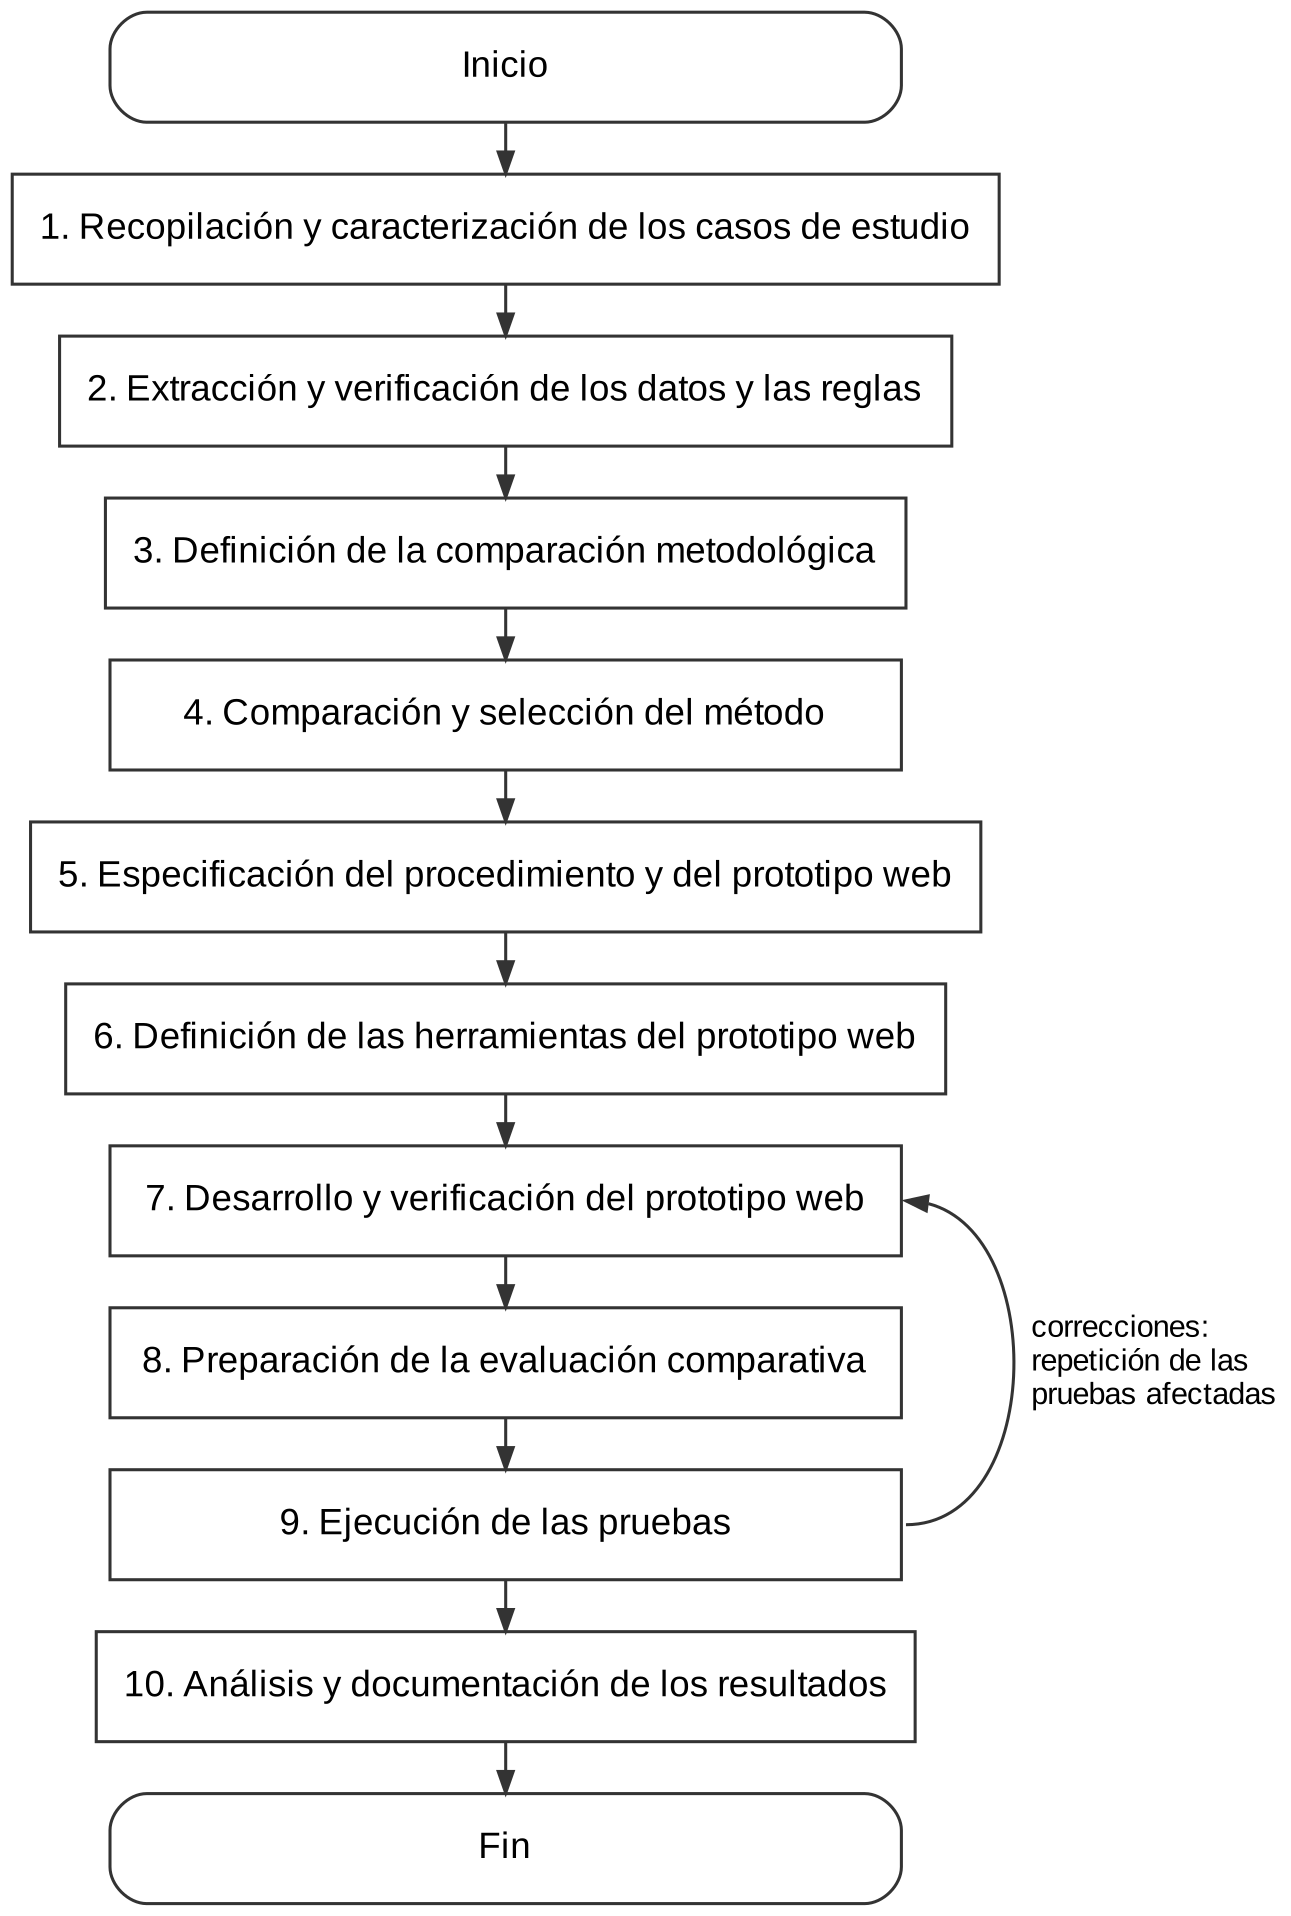
\includegraphics[height=0.62\textheight]{img/figura2.png}
\caption{Diagrama de flujo de las fases del trabajo.}
\label{fig:fases}
\end{figure}

\subsubsection{Fase 1: Recopilación y caracterización de los casos de estudio}

Los casos se seleccionarán mediante un muestreo no probabilístico intencional, a partir de la documentación pública disponible en el portal de la Dirección Nacional de Contrataciones Públicas y de la documentación de acceso público disponible en la página web de licitaciones del PTI [42]. Se considerarán procedimientos de distintos sectores y objetos de contratación, conforme a la delimitación del trabajo.

La unidad de análisis será el procedimiento de evaluación de un conjunto de ofertas que compitan por una misma unidad de adjudicación: ítem, lote o totalidad del llamado, según lo establecido en el pliego. Para las pruebas comparativas, cada observación corresponderá a la evaluación de un caso por un investigador en una modalidad determinada.

La selección considerará los siguientes requisitos:

\begin{itemize}
\item Correspondencia con el objeto y el periodo delimitados.
\item Disponibilidad de los pliegos y sus modificaciones aplicables.
\item Existencia de al menos dos ofertas admisibles y comparables.
\item Presencia de varios criterios que intervengan efectivamente en la valoración de las ofertas.
\item Información suficiente sobre los valores ofertados y las reglas necesarias para reconstruir la evaluación.
\end{itemize}

La existencia de varios requisitos técnicos obligatorios no se interpretará, por sí sola, como una evaluación multicriterio puntuable. Se distinguirán las condiciones de admisibilidad de los atributos que intervengan en la valoración y el ordenamiento.

Se utilizarán pliegos de bases y condiciones, adendas, actas de apertura, información pública de las ofertas, informes de evaluación y resoluciones de adjudicación. Los documentos se organizarán por procedimiento y se conservará su identificación, procedencia y fecha de consulta. La recopilación se realizará mediante una ficha documental, que registrará la institución, el identificador del llamado, el objeto de contratación, las fechas y los documentos disponibles.

Se elaborará un registro de los casos examinados, incluidos y excluidos, con sus respectivos motivos. La cantidad definitiva de casos se establecerá después de la revisión documental y antes de las pruebas, considerando la disponibilidad de información y los recursos del proyecto. Si no se obtuvieran casos suficientes, se informará esta limitación; los escenarios controlados no se presentarán como evidencia de contrataciones reales.

\textbf{Tareas:}

\begin{itemize}
\item \textbf{1.1.} Definición de los parámetros de búsqueda en el portal de la DNCP: objeto de contratación (distintos sectores y objetos, conforme a la delimitación), adjudicaciones de 2023 a 2026 y distintas instituciones públicas.
\item \textbf{1.2.} Descarga y organización por procedimiento de los documentos publicados en el portal de la DNCP y en la página web de licitaciones del PTI, incluido el reglamento de contrataciones del PTI si estuviera disponible, registrando su procedencia y fecha de consulta.
\item \textbf{1.3.} Elaboración de la ficha documental de cada procedimiento.
\item \textbf{1.4.} Verificación en cada procedimiento de los requisitos de selección e identificación de la unidad de adjudicación (ítem, lote o totalidad del llamado) y de las ofertas que compiten por ella.
\item \textbf{1.5.} Elaboración del registro de casos examinados, incluidos y excluidos, con el motivo de cada decisión, y anotación de la fecha de cierre de la recopilación.
\end{itemize}

\subsubsection{Fase 2: Extracción y verificación de los datos y las reglas}

La extracción se realizará mediante una matriz que relacionará cada oferta con sus datos, requisitos obligatorios, criterios de evaluación, escalas, reglas de puntuación, ponderaciones y condiciones de desempate, cuando correspondan.

Cada dato deberá vincularse con el documento y la ubicación que permitan comprobarlo. Uno de los investigadores realizará la extracción y el otro contrastará los registros con las fuentes originales. Las diferencias se resolverán antes de utilizar los casos en la evaluación.

La preparación comprenderá la revisión de valores faltantes, unidades de medida, formatos numéricos y duplicados. Las conversiones necesarias se documentarán y conservarán los valores originales. No se completará información ausente mediante suposiciones ni se utilizarán los requisitos mínimos solicitados como si fueran las características efectivamente ofertadas.

\textbf{Tareas:}

\begin{itemize}
\item \textbf{2.1.} Diseño de la matriz de extracción.
\item \textbf{2.2.} Extracción de los datos de las ofertas y de las reglas de evaluación, distinguiendo en cada pliego los requisitos obligatorios de admisibilidad de los atributos que intervienen en la puntuación y el ordenamiento, y vinculando cada dato con el documento y la ubicación donde puede comprobarse.
\item \textbf{2.3.} Verificación cruzada de los datos extraídos con las fuentes originales y resolución de las diferencias antes de utilizar cada caso.
\item \textbf{2.4.} Depuración de los datos (valores faltantes, unidades de medida, formatos numéricos y duplicados) y consolidación de los casos con información suficiente y datos verificados como conjunto disponible para las fases siguientes.
\end{itemize}

\subsubsection{Fase 3: Definición de la comparación metodológica}

Se elegirán los métodos candidatos entre los desarrollados en el marco teórico u otros que resulten pertinentes para los casos. Su inclusión se justificará a partir de las características de los casos y de las diferencias entre sus procedimientos, especificando la variante concreta de cada método.

Antes de efectuar la comparación, se establecerá una matriz que examine:

\begin{itemize}
\item Capacidad para representar los criterios, escalas y reglas de los pliegos.
\item Datos y parámetros requeridos.
\item Supuestos sobre las preferencias y la compensación entre criterios.
\item Interpretación de las ponderaciones.
\item Propiedades del ordenamiento.
\item Posibilidad de explicar y reproducir los resultados.
\item Viabilidad de implementación en el prototipo web.
\end{itemize}

Cada valoración se respaldará mediante documentación de los casos, bibliografía metodológica o análisis matemático. La compatibilidad con las reglas y la disponibilidad de los datos necesarios constituirán condiciones de admisibilidad metodológica; una mayor facilidad de programación no compensará su incumplimiento.

\textbf{Tareas:}

\begin{itemize}
\item \textbf{3.1.} Revisión de los métodos desarrollados en el marco teórico frente a las características de los casos y a la información disponible.
\item \textbf{3.2.} Elección de los métodos candidatos, con la justificación de su inclusión y la especificación de la variante concreta de cada uno.
\item \textbf{3.3.} Elaboración de la matriz de comparación con los criterios establecidos.
\end{itemize}

\subsubsection{Fase 4: Comparación y selección de los métodos}

Cuando exista información suficiente, se realizarán aplicaciones numéricas para examinar el comportamiento de los métodos. Los parámetros que no puedan justificarse con la documentación se identificarán como supuestos de escenarios controlados y no como reglas de la contratación estudiada.

La selección se fundamentará en la adecuación al problema y en las propiedades verificadas. La coincidencia con un adjudicatario histórico se utilizará como información de contraste, sin considerarla una demostración suficiente de superioridad. Tampoco se estimarán ponderaciones a partir del ganador para sustituir las reglas documentadas del pliego.

\textbf{Tareas:}

\begin{itemize}
\item \textbf{4.1.} Llenado de la matriz de comparación para los métodos candidatos, respaldando cada valoración con su fuente, y clasificación de la compatibilidad de cada método con los datos disponibles como compatible, incompatible o no determinable.
\item \textbf{4.2.} Realización de aplicaciones numéricas con los casos de información suficiente para examinar el comportamiento de los métodos.
\item \textbf{4.3.} Selección de los métodos y justificación de cada uno a partir de la adecuación al problema y de las propiedades verificadas.
\end{itemize}

\subsubsection{Fase 5: Especificación del procedimiento y del prototipo web}

Se definirán las entradas, las transformaciones, las funciones de puntuación, la agregación de resultados y las condiciones de desempate de cada procedimiento seleccionado. También se establecerán la precisión numérica y las reglas de redondeo.

Se examinarán la monotonía ante mejoras en los criterios, el tratamiento de ofertas dominadas, la invariancia frente al orden de ingreso y el comportamiento del ordenamiento al incorporar o retirar alternativas no ganadoras. Para cada propiedad se explicitarán los supuestos bajo los cuales se espera su cumplimiento. Asimismo, se realizará un análisis de sensibilidad de las clasificaciones ante variaciones de las ponderaciones y de los parámetros, distinguiendo los valores documentados en los pliegos de los supuestos de escenarios controlados.

Las afirmaciones generales se sustentarán mediante demostraciones o se refutarán mediante contraejemplos. Las pruebas numéricas servirán para comprobar situaciones particulares y detectar errores de implementación. Los resultados se registrarán como propiedades demostradas bajo condiciones explícitas, refutadas o pendientes de justificación.

El prototipo web permitirá registrar los casos y las ofertas, distinguir requisitos obligatorios de criterios puntuables, configurar las reglas documentadas, ejecutar los métodos seleccionados y consultar la clasificación resultante. También permitirá examinar los valores intermedios y las evidencias asociadas a cada resultado.

Se utilizará una arquitectura cliente-servidor con separación entre presentación, lógica de evaluación y almacenamiento. La interfaz gestionará la interacción con el usuario; la lógica de evaluación aplicará las reglas y los cálculos; y la capa de almacenamiento conservará los datos y las ejecuciones. Esta separación permitirá verificar el motor de cálculo de forma independiente de la interfaz. La Figura 2 presenta el diagrama funcional del prototipo web.



\begin{figure}[H]
\centering
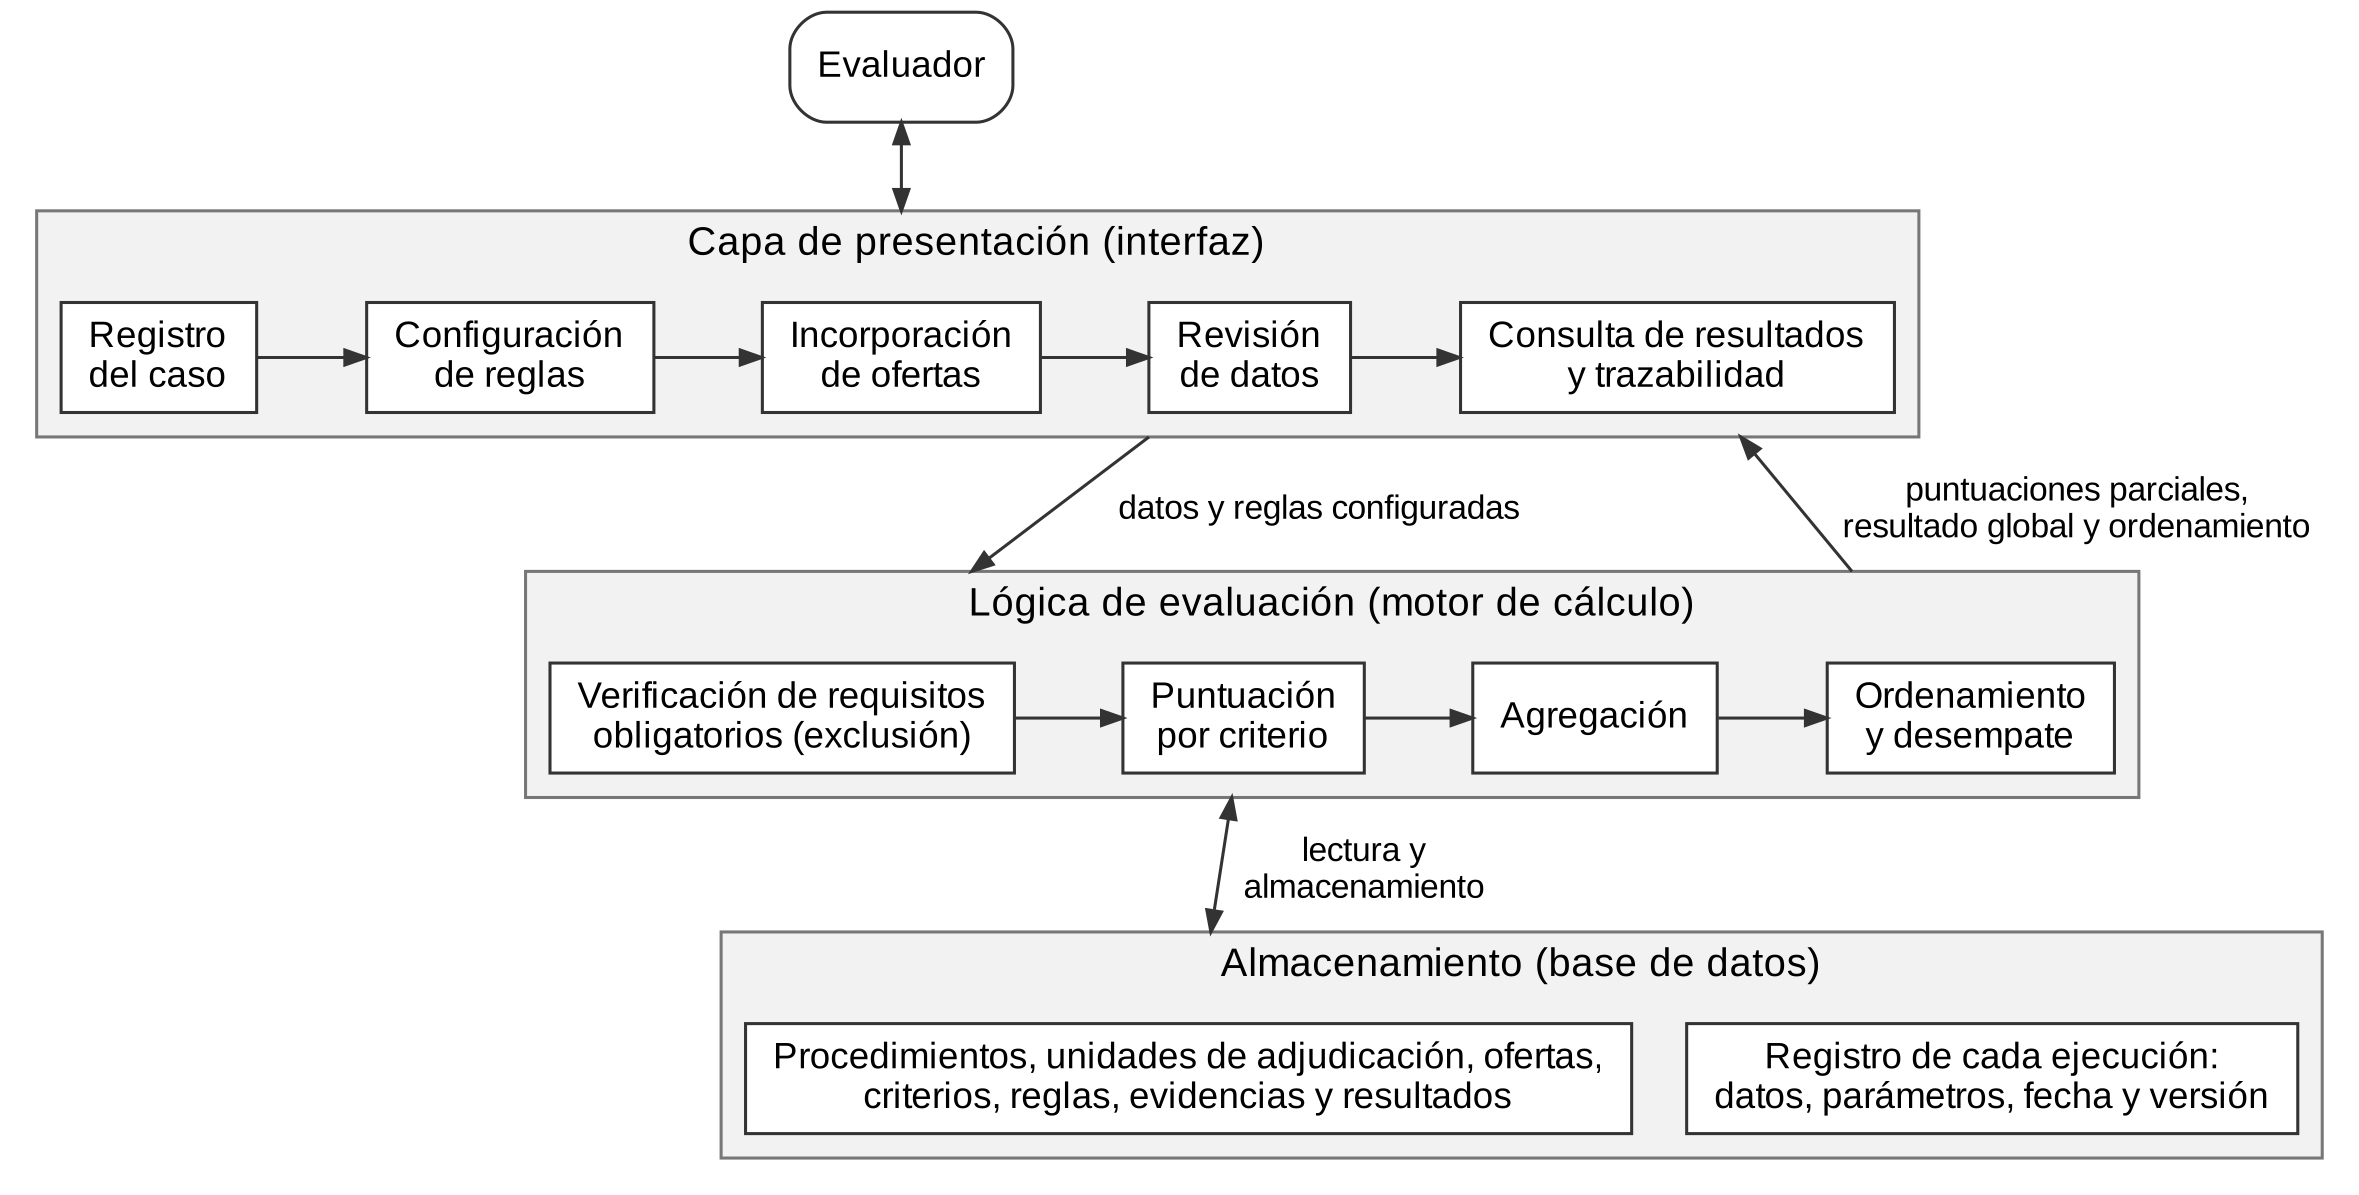
\includegraphics[width=0.95\linewidth]{img/figura1.png}
\caption{Diagrama funcional del prototipo web.}
\label{fig:funcional}
\end{figure}

La base de datos relacionará procedimientos, unidades de adjudicación, ofertas, criterios, reglas, evidencias y resultados. Cada ejecución conservará una copia identificable de los datos y parámetros utilizados, junto con la fecha y la versión del prototipo web, de manera que las modificaciones posteriores no alteren el registro de evaluaciones anteriores.

La navegación seguirá la secuencia de registro del caso, configuración de reglas, incorporación de ofertas, revisión de datos y consulta de resultados. Los formularios incluirán etiquetas claras, unidades de medida, indicaciones sobre campos obligatorios y mensajes que permitan localizar y corregir errores.

La pantalla de resultados mostrará las puntuaciones parciales, el resultado global y el ordenamiento. Desde cada puntuación se podrá consultar el dato de entrada, la regla aplicada y la evidencia correspondiente. Los empates o las situaciones no resueltas por las reglas registradas se mostrarán expresamente.

\textbf{Tareas:}

\begin{itemize}
\item \textbf{5.1.} Definición del procedimiento de cada método seleccionado: entradas, transformaciones, funciones de puntuación, agregación, condiciones de desempate, precisión numérica y reglas de redondeo.
\item \textbf{5.2.} Formulación de las propiedades a verificar y de sus supuestos, demostración o refutación de cada una mediante contraejemplos y registro de su estado (demostrada bajo condiciones explícitas, refutada o pendiente de justificación).
\item \textbf{5.3.} Análisis de sensibilidad de las clasificaciones ante variaciones de las ponderaciones y de los parámetros de cada método seleccionado.
\item \textbf{5.4.} Definición de los requerimientos del prototipo web.
\item \textbf{5.5.} Diseño de la arquitectura cliente-servidor, con separación entre presentación, lógica de evaluación y almacenamiento.
\item \textbf{5.6.} Diseño de la base de datos y del registro de cada ejecución con sus datos, parámetros, fecha y versión del prototipo web.
\item \textbf{5.7.} Diseño de la interfaz: secuencia de navegación, formularios y pantalla de resultados.
\end{itemize}

\subsubsection{Fase 6: Definición de las herramientas del prototipo web}

Las herramientas de desarrollo (lenguajes de programación, frameworks, gestor de base de datos y herramientas de prueba) se definirán después de establecer los requerimientos y la arquitectura. Su selección considerará la compatibilidad con la arquitectura cliente-servidor y con los requerimientos del prototipo web, la posibilidad de probar el motor de cálculo de forma independiente de la interfaz, el soporte para conservar el registro de las ejecuciones y la disponibilidad de documentación y de licencias de uso. Cada elección se justificará frente a las alternativas revisadas.

\textbf{Tareas:}

\begin{itemize}
\item \textbf{6.1.} Revisión de alternativas de lenguajes de programación, frameworks, gestores de bases de datos y herramientas de prueba compatibles con la arquitectura cliente-servidor.
\item \textbf{6.2.} Selección de las herramientas y justificación de cada elección según los requisitos técnicos derivados de los requerimientos y de la arquitectura definidos.
\item \textbf{6.3.} Configuración del entorno de desarrollo y del control de versiones.
\end{itemize}

\subsubsection{Fase 7: Desarrollo y verificación del prototipo web}

El desarrollo será incremental. Primero se implementará el registro de datos; luego, el motor de evaluación; y finalmente, la consulta de resultados y su trazabilidad. Cada incremento se verificará antes de integrarse con los restantes componentes.

Se realizarán pruebas unitarias del motor de cálculo, pruebas de integración entre los componentes y pruebas funcionales de los requerimientos previstos. Se examinarán escenarios con empates, valores límite, datos faltantes, incumplimientos obligatorios y distintas cantidades de ofertas y criterios.

Los resultados se contrastarán con cálculos de referencia elaborados de forma independiente del código del prototipo web y revisados antes de las mediciones. Las discrepancias se analizarán considerando las reglas de puntuación y la precisión establecida.

La interacción se revisará mediante tareas de registro, corrección y consulta, documentando errores de navegación y dificultades observadas. Si esta revisión se realiza únicamente con los investigadores, sus resultados se limitarán a una comprobación interna de uso.

\textbf{Tareas:}

\begin{itemize}
\item \textbf{7.1.} Desarrollo del registro de datos (casos, ofertas, criterios, reglas y evidencias).
\item \textbf{7.2.} Desarrollo del motor de evaluación, separado de la interfaz: exclusión por requisitos obligatorios, puntuación, agregación, ordenamiento y desempate.
\item \textbf{7.3.} Desarrollo de la consulta de resultados y su trazabilidad.
\item \textbf{7.4.} Elaboración y revisión de los cálculos de referencia independientes del código del prototipo web.
\item \textbf{7.5.} Realización de pruebas unitarias, de integración y funcionales, y análisis de las discrepancias con los cálculos de referencia.
\item \textbf{7.6.} Revisión de la interacción mediante tareas de registro, corrección y consulta.
\end{itemize}

\subsubsection{Fase 8: Preparación de la evaluación comparativa}

El conjunto de prueba comprenderá los casos reconstruidos en las Fases 1 y 2 y escenarios controlados, identificados como tales, diseñados para examinar situaciones que los casos no presenten, como empates, valores límite o la incorporación y el retiro de ofertas no ganadoras. La comparación entre la modalidad manual y la automatizada, en tiempo de evaluación y errores de cálculo, se realizará con los casos reconstruidos; la correcta aplicación de los métodos implementados y la reproducibilidad de los cálculos se verificarán con ambos tipos de prueba.

Se propone que los dos investigadores ejecuten ambas modalidades. La modalidad manual utilizará una ficha de evaluación y una calculadora básica; la automatizada empleará el prototipo web. Ambas exigirán los mismos resultados y el mismo nivel de documentación. En la comparación manual–automatizada, cada caso se evaluará con un único método, el que, según la comparación de la Fase 4, mejor represente las reglas de su pliego, y ambas modalidades aplicarán ese mismo método con las mismas reglas; esta asignación se registrará antes de las pruebas. Las comprobaciones de correcta aplicación y de reproducibilidad, en cambio, se realizarán con cada uno de los métodos seleccionados.

Se realizará una práctica previa con un caso ajeno al conjunto de medición. El orden de las modalidades se alternará entre investigadores y casos, procurando equilibrar las secuencias manual–automatizada y automatizada–manual. Durante la segunda ejecución no se consultarán las respuestas de la primera.

El tiempo se medirá desde la entrega del conjunto de datos verificados hasta la obtención de la clasificación y el registro de sus fundamentos. Se incluirán la carga o transcripción de datos y las correcciones realizadas durante la tarea. La búsqueda documental y la preparación previa de los casos quedarán fuera de ambas mediciones.

Antes de iniciar las pruebas se establecerán el número de casos y escenarios controlados, las sesiones, las repeticiones y su distribución. Las repeticiones se identificarán como observaciones de un mismo caso e investigador, evitando tratarlas como casos independientes.

Para la reproducibilidad, en cada caso o escenario y con cada método seleccionado se obtendrán dos pares de ejecuciones: cada investigador realizará una ejecución original en el prototipo web y el otro investigador la reejecutará una vez, en una sesión posterior, a partir del registro guardado de esa ejecución (datos, parámetros y versión del prototipo web), sin volver a ingresar los datos.

La valoración por evaluadores expertos complementará las mediciones anteriores. Se convocará a evaluadores con experiencia en licitaciones públicas, externos al equipo de desarrollo, y se elaborará un cuestionario con escala Likert de 1 a 5 organizado en tres dimensiones: fidelidad de las reglas implementadas respecto de los pliegos, comprensión de la trazabilidad de los resultados y utilidad percibida del prototipo web. Las respuestas se registrarán sin datos que permitan identificar a los evaluadores.

Antes de la comparación manual–automatizada se fijarán la versión del prototipo web, los casos, los resultados de referencia y los instrumentos de medición. Las correcciones posteriores se documentarán y requerirán repetir las pruebas afectadas.

\textbf{Tareas:}

\begin{itemize}
\item \textbf{8.1.} Establecimiento del número de casos reconstruidos y escenarios controlados, las sesiones, las repeticiones y su distribución; asignación a cada caso del método con el que se realizará la comparación manual–automatizada; y fijación de las reejecuciones para la reproducibilidad: una reejecución de cada ejecución original, a cargo del otro investigador, lo que da dos pares de ejecuciones por caso o escenario y por método seleccionado.
\item \textbf{8.2.} Elaboración de los instrumentos: ficha de evaluación manual, registro de tiempos, registro de errores y lista de comprobación de trazabilidad.
\item \textbf{8.3.} Realización de una práctica previa con un caso ajeno al conjunto de medición y fijación de la versión del prototipo web, los casos, los resultados de referencia y los instrumentos.
\item \textbf{8.4.} Selección de evaluadores con experiencia en licitaciones públicas, externos al equipo, y diseño de un cuestionario con escala Likert de 1 a 5 sobre la fidelidad de las reglas implementadas, la comprensión de la trazabilidad y la utilidad percibida.
\end{itemize}

\subsubsection{Fase 9: Ejecución de las pruebas}

El tiempo de evaluación se registrará en minutos por caso y modalidad. Se registrará también el tiempo de procesamiento del prototipo web para los casos de prueba, diferenciándolo del tiempo total que necesita una persona para completar la evaluación. Los errores de cálculo se determinarán mediante el contraste de un conjunto previamente definido de resultados numéricos con los valores de referencia. Se registrarán su cantidad y su proporción respecto del total revisado, diferenciando errores aritméticos, de transcripción y de configuración.

La trazabilidad se examinará mediante una lista de comprobación común a ambas modalidades. Un resultado tendrá trazabilidad completa cuando permita identificar la oferta, el dato de entrada, la fuente, la regla y los parámetros utilizados, así como las operaciones necesarias para reconstruirlo. Se calculará la proporción de resultados que cumplan todos estos elementos.

La correcta aplicación de los métodos implementados se expresará, para cada método, mediante la proporción de pruebas concordantes con los cálculos de referencia, con los casos reconstruidos y los escenarios controlados. La reproducibilidad se comprobará reejecutando cada ejecución original desde su registro guardado, en otra sesión y a cargo del otro investigador, conforme a lo establecido en la tarea 8.1. Dos ejecuciones se considerarán equivalentes cuando produzcan el mismo ordenamiento y las mismas puntuaciones parciales y globales, con la precisión numérica y las reglas de redondeo definidas en la tarea 5.1. Se calculará el porcentaje de pares equivalentes por método.

Finalmente, se realizará una sesión de uso del prototipo web con uno o dos casos reconstruidos junto a los evaluadores expertos, quienes responderán el cuestionario elaborado en la tarea 8.4. Se registrarán sus valoraciones y observaciones sin datos que permitan identificarlos.

\textbf{Tareas:}

\begin{itemize}
\item \textbf{9.1.} Ejecución de cada caso reconstruido en ambas modalidades, con el método asignado en la tarea 8.1, y registro del tiempo de evaluación, del tiempo de procesamiento del prototipo web y de la trazabilidad de cada ejecución.
\item \textbf{9.2.} Contraste de los resultados numéricos con los valores de referencia y recuento de los errores de cálculo.
\item \textbf{9.3.} Comprobación de la correcta aplicación de cada método implementado mediante el contraste con los cálculos de referencia, con los casos reconstruidos y los escenarios controlados.
\item \textbf{9.4.} Comprobación de la reproducibilidad: reejecución de cada ejecución original desde su registro guardado, en otra sesión y a cargo del otro investigador, y verificación de la equivalencia de cada par (mismo ordenamiento y mismas puntuaciones parciales y globales, con la precisión y el redondeo de la tarea 5.1), por método.
\item \textbf{9.5.} Sesión de uso del prototipo web con uno o dos casos reconstruidos junto a los evaluadores expertos, aplicación del cuestionario y registro de sus observaciones.
\end{itemize}

\subsubsection{Fase 10: Análisis y documentación de los resultados}

El análisis será descriptivo y comparativo. Se presentarán conteos, porcentajes, medianas, rangos y diferencias por pares correspondientes al mismo caso e investigador. Las reducciones relativas se calcularán únicamente cuando el valor de la modalidad manual sea mayor que cero. Las diferencias de trazabilidad se expresarán en puntos porcentuales. La correcta aplicación y la reproducibilidad se informarán por método. La valoración de los evaluadores expertos se resumirá mediante la mediana por dimensión y el porcentaje de ítems con valoración igual o superior a 4, acompañados de sus observaciones cualitativas, sin datos que permitan identificar a los evaluadores.

Los componentes de la hipótesis se examinarán por separado. Una disminución del tiempo no se interpretará como evidencia de reducción de errores, y la ausencia de errores en ambas modalidades indicará igualdad en esa medición. Los casos reconstruidos y los escenarios controlados se analizarán separadamente. Asimismo, los casos procedentes de la DNCP y del PTI se presentarán por separado, debido a que responden a regímenes normativos distintos.

Las conclusiones considerarán el número de casos, su selección intencional, el aprendizaje y la participación de los propios desarrolladores. Los resultados permitirán valorar el prototipo web en las condiciones estudiadas, sin extrapolar directamente su desempeño al de los comités evaluadores de las instituciones públicas.

\textbf{Tareas:}

\begin{itemize}
\item \textbf{10.1.} Cálculo de las medidas descriptivas, de las diferencias por pares entre modalidades, de los indicadores de correcta aplicación y reproducibilidad por método y del resumen de la valoración de los evaluadores expertos.
\item \textbf{10.2.} Contraste de cada componente de la hipótesis con los resultados obtenidos.
\item \textbf{10.3.} Descripción de las limitaciones y redacción de los resultados, los alcances y las conclusiones.
\end{itemize}

\subsection{Cronograma de tareas}



Las tareas descritas en los apartados 8.1.2 a 8.1.11, cuya secuencia por fases se representa en la Figura 1, se distribuyen en el cronograma de la Tabla 1.

\begin{landscape}
\begin{center}
\begin{longtable}{>{\raggedright\arraybackslash}p{7.5cm} >{\centering\arraybackslash}p{1.3cm} >{\centering\arraybackslash}p{1.3cm} >{\centering\arraybackslash}p{1.3cm} >{\centering\arraybackslash}p{1.3cm} >{\centering\arraybackslash}p{1.3cm} >{\centering\arraybackslash}p{1.3cm} >{\centering\arraybackslash}p{1.3cm} >{\centering\arraybackslash}p{1.3cm}}
\caption{Cronograma de tareas.}\label{tab:cronograma}\\
\toprule
\textbf{Fase / tarea (Inicio: 01/01/2027 – Cierre: 31/08/2027)} & \textbf{Ene} & \textbf{Feb} & \textbf{Mar} & \textbf{Abr} & \textbf{May} & \textbf{Jun} & \textbf{Jul} & \textbf{Ago} \\
\midrule
\endfirsthead
\multicolumn{9}{l}{\textit{Tabla 1 (continuación): Cronograma de tareas.}}\\
\toprule
\textbf{Fase / tarea (Inicio: 01/01/2027 – Cierre: 31/08/2027)} & \textbf{Ene} & \textbf{Feb} & \textbf{Mar} & \textbf{Abr} & \textbf{May} & \textbf{Jun} & \textbf{Jul} & \textbf{Ago} \\
\midrule
\endhead
\midrule
\multicolumn{9}{r}{\textit{Continúa en la página siguiente}}\\
\endfoot
\bottomrule
\endlastfoot
\textbf{1. Recopilación y caracterización de los casos de estudio} & \textbf{X} &  &  &  &  &  &  &  \\
1.1. Parámetros de búsqueda en el portal de la DNCP & X &  &  &  &  &  &  &  \\
1.2. Descarga y organización de la documentación (DNCP y PTI) & X &  &  &  &  &  &  &  \\
1.3. Ficha documental de cada procedimiento & X &  &  &  &  &  &  &  \\
1.4. Verificación de requisitos de selección y unidad de adjudicación & X &  &  &  &  &  &  &  \\
1.5. Registro de casos incluidos y excluidos & X &  &  &  &  &  &  &  \\
\textbf{2. Extracción y verificación de los datos y las reglas} & \textbf{X} & \textbf{X} &  &  &  &  &  &  \\
2.1. Diseño de la matriz de extracción & X &  &  &  &  &  &  &  \\
2.2. Extracción de datos y reglas de evaluación & X & X &  &  &  &  &  &  \\
2.3. Verificación cruzada con las fuentes &  & X &  &  &  &  &  &  \\
2.4. Depuración y consolidación de los casos &  & X &  &  &  &  &  &  \\
\textbf{3. Definición de la comparación metodológica} &  & \textbf{X} & \textbf{X} &  &  &  &  &  \\
3.1. Revisión de los métodos frente a los casos &  & X &  &  &  &  &  &  \\
3.2. Elección de los métodos candidatos y sus variantes &  & X &  &  &  &  &  &  \\
3.3. Elaboración de la matriz de comparación &  &  & X &  &  &  &  &  \\
\textbf{4. Comparación y selección de los métodos} &  &  & \textbf{X} & \textbf{X} &  &  &  &  \\
4.1. Llenado de la matriz y clasificación de compatibilidad &  &  & X &  &  &  &  &  \\
4.2. Aplicaciones numéricas &  &  & X & X &  &  &  &  \\
4.3. Selección de los métodos y justificación de cada uno &  &  &  & X &  &  &  &  \\
\textbf{5. Especificación del procedimiento y del prototipo web} &  &  &  & \textbf{X} &  &  &  &  \\
5.1. Definición del procedimiento de cada método seleccionado &  &  &  & X &  &  &  &  \\
5.2. Propiedades: formulación, demostración o refutación &  &  &  & X &  &  &  &  \\
5.3. Análisis de sensibilidad &  &  &  & X &  &  &  &  \\
5.4. Requerimientos del prototipo web &  &  &  & X &  &  &  &  \\
5.5. Diseño de la arquitectura &  &  &  & X &  &  &  &  \\
5.6. Diseño de la base de datos &  &  &  & X &  &  &  &  \\
5.7. Diseño de la interfaz &  &  &  & X &  &  &  &  \\
\textbf{6. Definición de las herramientas del prototipo web} &  &  &  & \textbf{X} & \textbf{X} &  &  &  \\
6.1. Revisión de alternativas tecnológicas &  &  &  & X &  &  &  &  \\
6.2. Selección y justificación de las herramientas &  &  &  &  & X &  &  &  \\
6.3. Configuración del entorno y control de versiones &  &  &  &  & X &  &  &  \\
\textbf{7. Desarrollo y verificación del prototipo web} &  &  &  &  & \textbf{X} & \textbf{X} &  &  \\
7.1. Desarrollo del registro de datos &  &  &  &  & X &  &  &  \\
7.2. Desarrollo del motor de evaluación &  &  &  &  & X & X &  &  \\
7.3. Desarrollo de la consulta de resultados y trazabilidad &  &  &  &  &  & X &  &  \\
7.4. Cálculos de referencia independientes &  &  &  &  & X &  &  &  \\
7.5. Pruebas unitarias, de integración y funcionales &  &  &  &  & X & X &  &  \\
7.6. Revisión de la interacción &  &  &  &  &  & X &  &  \\
\textbf{8. Preparación de la evaluación comparativa} &  &  &  &  &  & \textbf{X} & \textbf{X} &  \\
8.1. Casos y escenarios, sesiones, repeticiones, método por caso y reejecuciones &  &  &  &  &  & X &  &  \\
8.2. Elaboración de los instrumentos &  &  &  &  &  & X &  &  \\
8.3. Práctica previa y fijación de versión, casos e instrumentos &  &  &  &  &  &  & X &  \\
8.4. Selección de expertos y diseño del cuestionario Likert &  &  &  &  &  &  & X &  \\
\textbf{9. Ejecución de las pruebas} &  &  &  &  &  &  & \textbf{X} &  \\
9.1. Ejecución de los casos en ambas modalidades &  &  &  &  &  &  & X &  \\
9.2. Contraste con la referencia y recuento de errores &  &  &  &  &  &  & X &  \\
9.3. Comprobación de la correcta aplicación de los métodos &  &  &  &  &  &  & X &  \\
9.4. Comprobación de la reproducibilidad por método &  &  &  &  &  &  & X &  \\
9.5. Sesión de uso del prototipo web con los expertos &  &  &  &  &  &  & X &  \\
\textbf{10. Análisis y documentación de los resultados} &  &  &  &  &  &  & \textbf{X} & \textbf{X} \\
10.1. Medidas descriptivas y diferencias por pares &  &  &  &  &  &  & X & X \\
10.2. Contraste de los componentes de la hipótesis &  &  &  &  &  &  &  & X \\
10.3. Limitaciones, resultados y conclusiones &  &  &  &  &  &  &  & X \\
\end{longtable}
\end{center}
\end{landscape}
\subsection{Operacionalización de variables}

\begin{enumerate}
\item \textbf{Completitud documental de las licitaciones:} Grado en que los documentos de cada caso permiten reconstruir su evaluación. Indicador: cantidad y porcentaje de casos revisados con información suficiente (pliego, datos de las ofertas, informe de evaluación y adjudicación).
\item \textbf{Parámetros y reglas de evaluación:} Requisitos obligatorios, criterios, escalas, reglas de puntuación y ponderaciones documentados en cada caso. Indicador: tipo y cantidad de requisitos y criterios, escalas y reglas registradas, con la fuente documental de cada elemento.
\item \textbf{Compatibilidad y comportamiento de los métodos multicriterio:} Correspondencia de cada método con las reglas de los pliegos, los datos disponibles y las propiedades exigidas. Indicador: compatibilidad con los datos (compatible, incompatible o no determinable) y estado de cada propiedad (demostrada bajo supuestos, refutada o pendiente).
\item \textbf{Cobertura técnica de las herramientas:} Conjunto de lenguajes de programación, frameworks, gestor de base de datos y herramientas de prueba definidos para el desarrollo del prototipo web. Indicador: herramientas seleccionadas y documentadas con su justificación, y porcentaje de requisitos técnicos cubiertos por ellas.
\item \textbf{Operatividad funcional del prototipo:} Grado en que el prototipo web realiza las funciones previstas de registro, cálculo y consulta. Indicador: porcentaje de funciones verificadas satisfactoriamente respecto de las previstas.
\item \textbf{Correcta aplicación de los métodos:} Concordancia de los resultados del prototipo web, para cada método implementado, con cálculos de referencia elaborados de forma independiente, en casos reconstruidos y escenarios controlados. Indicador: porcentaje de pruebas concordantes con la referencia, por método.
\item \textbf{Reproducibilidad de los resultados:} Obtención de resultados equivalentes al reejecutar cada ejecución original desde su registro guardado, en otra sesión y a cargo del otro investigador. Se consideran equivalentes dos ejecuciones con el mismo ordenamiento y las mismas puntuaciones parciales y globales, con la precisión numérica y las reglas de redondeo de la tarea 5.1. Indicador: porcentaje de pares equivalentes, por método.
\item \textbf{Nivel de trazabilidad:} Posibilidad de identificar, para cada resultado, la oferta, el dato de entrada, la fuente, la regla, los parámetros y las operaciones utilizadas. Indicador: porcentaje de resultados con trazabilidad completa según la lista de comprobación común a ambas modalidades.
\item \textbf{Duración de la evaluación:} Duración desde la entrega del conjunto de datos verificados hasta la obtención de la clasificación y el registro de sus fundamentos. Indicador: minutos por caso y modalidad.
\item \textbf{Frecuencia de errores:} Discrepancias entre los resultados numéricos obtenidos y los valores de referencia. Indicador: cantidad y proporción de errores respecto del total revisado, por tipo (aritméticos, de transcripción y de configuración).
\item \textbf{Validación de expertos:} Valoración del prototipo web por evaluadores con experiencia en licitaciones públicas, externos al equipo de desarrollo, mediante un cuestionario con escala Likert de 1 a 5 sobre la fidelidad de las reglas implementadas, la comprensión de la trazabilidad y la utilidad percibida. Indicador: mediana de valoración por dimensión (escala 1-5) y porcentaje de ítems con valoración $\geq 4$, más observaciones cualitativas registradas.
\end{enumerate}

La Tabla 2 relaciona cada objetivo específico con sus tareas, variables e indicadores.

\begin{center}
\setlength{\tabcolsep}{4pt}
\begin{longtable}{>{\raggedright\arraybackslash}p{2.1cm} >{\raggedright\arraybackslash}p{2.7cm} >{\raggedright\arraybackslash}p{2.1cm} >{\raggedright\arraybackslash}p{4.3cm}}
\caption{Operacionalización de variables.}\label{tab:operacionalizacion}\\
\toprule
\textbf{Objetivo específico} & \textbf{Tarea} & \textbf{Variable} & \textbf{Indicador / estimador / definición operacional} \\
\midrule
\endfirsthead
\multicolumn{4}{l}{\textit{Tabla 2 (continuación): Operacionalización de variables.}}\\
\toprule
\textbf{Objetivo específico} & \textbf{Tarea} & \textbf{Variable} & \textbf{Indicador / estimador / definición operacional} \\
\midrule
\endhead
\midrule
\multicolumn{4}{r}{\textit{Continúa en la página siguiente}}\\
\endfoot
\bottomrule
\endlastfoot
1. Identificar y seleccionar los casos de estudio de licitaciones públicas que cuenten con información documental suficiente para su reconstrucción. & Recopilación y caracterización de los casos de estudio (Fase 1, tareas 1.1 a 1.5). & Completitud documental de las licitaciones. & Cantidad y porcentaje de casos revisados con información suficiente: pliego, datos de las ofertas, informe de evaluación y adjudicación. \\
\addlinespace
2. Identificar los requisitos obligatorios, criterios de evaluación, escalas, reglas de puntuación o ponderaciones, a partir de los documentos de los casos seleccionados. & Extracción y verificación de los datos y las reglas (Fase 2, tareas 2.1 a 2.4). & Parámetros y reglas de evaluación. & Tipo y cantidad de requisitos y criterios. Escalas y reglas de puntuación documentadas. Ponderaciones registradas, cuando correspondan. Fuente documental de cada elemento. \\
\addlinespace
3. Comparar métodos de decisión multicriterio mediante su aplicación a los casos seleccionados, para justificar la elección de los más adecuados según los criterios de comparación establecidos. & Definición de la comparación metodológica; comparación y selección de los métodos (Fases 3 y 4, tareas 3.1 a 4.3); especificación de los procedimientos, propiedades y análisis de sensibilidad (Fase 5, tareas 5.1 a 5.3). & Compatibilidad y comportamiento de los métodos multicriterio. & Compatibilidad con los datos disponibles: compatible, incompatible o no determinable. Propiedades examinadas: demostradas bajo supuestos, refutadas o pendientes. Métodos seleccionados y justificación. Análisis de sensibilidad: variación de las clasificaciones ante cambios en las ponderaciones y los parámetros. \\
\addlinespace
4. Definir la arquitectura y las herramientas tecnológicas necesarias para el desarrollo del prototipo web de soporte a la decisión. & Requerimientos, arquitectura, base de datos e interfaz del prototipo web (Fase 5, tareas 5.4 a 5.7); definición de las herramientas del prototipo web (Fase 6, tareas 6.1 a 6.3). & Cobertura técnica de las herramientas. & Herramientas seleccionadas y documentadas con su justificación. Porcentaje de requisitos técnicos cubiertos por las herramientas seleccionadas. \\
\addlinespace
5. Implementar un prototipo web para el apoyo a la toma de decisión en las licitaciones. & Desarrollo y verificación del prototipo web (Fase 7, tareas 7.1 a 7.6). & Operatividad funcional del prototipo. & Porcentaje de funciones verificadas satisfactoriamente respecto de las previstas: registro de ofertas, criterios, parámetros y evidencias; cálculo y consulta de resultados. \\
\addlinespace
6. Evaluar el prototipo web con los casos reconstruidos y con escenarios controlados, verificando la correcta aplicación de los métodos implementados, la reproducibilidad de los cálculos y la trazabilidad de los resultados, y comparando el tiempo de evaluación y los errores de cálculo con la aplicación manual de las mismas reglas, con la valoración de evaluadores expertos ajenos al equipo. & Preparación de la evaluación comparativa y de la validación de expertos; ejecución de las pruebas y sesión de uso con los expertos; análisis y documentación de los resultados (Fases 8 a 10, tareas 8.1 a 10.3, incluidas 8.4 y 9.5). & Correcta aplicación de los métodos. Reproducibilidad de los resultados. Nivel de trazabilidad. Duración de la evaluación. Frecuencia de errores. Validación de expertos. & Correcta aplicación: porcentaje de pruebas concordantes con el cálculo de referencia, por método, en casos reconstruidos y escenarios controlados. Reproducibilidad: porcentaje de pares equivalentes, por método (reejecución desde el registro guardado, en otra sesión y a cargo del otro investigador; equivalencia: mismo ordenamiento y mismas puntuaciones parciales y globales, con la precisión y el redondeo de la tarea 5.1). Trazabilidad: porcentaje de resultados con trazabilidad completa según la lista de comprobación común a ambas modalidades. Duración: minutos por caso y modalidad. Frecuencia de errores: cantidad y proporción por tipo (aritméticos, de transcripción y de configuración). Validación de expertos: mediana de valoración por dimensión (escala 1-5) y porcentaje de ítems con valoración $\geq 4$, más observaciones cualitativas registradas. \\
\addlinespace
\end{longtable}
\end{center}
\clearpage
\section*{Referencias Bibliográficas}
\addcontentsline{toc}{section}{Referencias Bibliográficas}
\begin{reflist}

\item[] [1] República del Paraguay, ``Ley N.º 7021/2022, de Suministro y Contrataciones Públicas,'' 9 dic. 2022. Accedido: 24 de agosto de 2026. [En línea]. Disponible en: \url{https://www.contrataciones.gov.py/buscador/marco-legal.html?nro_nombre=7021}

\item[] [2] Presidencia de la República del Paraguay, ``Decreto N.º 2264/2024, Reglamentación de la Ley N.º 7021/22 del 9 de diciembre de 2022, `De Suministro y Contrataciones Públicas,''' 1 ag. 2024. Accedido: 24 de agosto de 2026. [En línea]. Disponible en: \url{https://www.contrataciones.gov.py/buscador/marco-legal.html?nro_nombre=2264}

\item[] [3] J.-M. Lehtonen y K. Virtanen, ``Choosing the most economically advantageous tender using a multi-criteria decision analysis approach,'' J. Public Procure., vol. 22, no. 2, pp. 164-179, mzo. 2022. [En línea]. Disponible en: \url{https://doi.org/10.1108/JOPP-06-2021-0040}

\item[] [4] F. Schotanus, G. van den Engh, Y. Nijenhuis y J. Telgen, ``Supplier selection with rank reversal in public tenders,'' J. Purch. Supply Manag., vol. 28, no. 2, art. no. 100744, mzo. 2022. [En línea]. Disponible en: \url{https://doi.org/10.1016/j.pursup.2021.100744}

\item[] [5] OECD, ``Size of public procurement,'' Government at a Glance 2023, oecd.org. Accedido: 3 de noviembre de 2026. [En línea]. Disponible en: \url{https://www.oecd.org/en/publications/government-at-a-glance-2023_3d5c5d31-en/full-report/component-36.html}

\item[] [6] D. Anelli, P. Morano, T. Acquafredda y F. Tajani, ``Structuring multi-criteria decision approaches for public procurement: methods, standards and applications,'' Systems, vol. 13, no. 9, art. no. 777, sept. 2025. [En línea]. Disponible en: \url{https://doi.org/10.3390/systems13090777}

\item[] [7] P.-L. Poon, M. F. Lau, Y. T. Yu y S.-F. Tang, ``Spreadsheet quality assurance: a literature review,'' Front. Comput. Sci., vol. 18, no. 2, art. no. 182203, abr. 2024. [En línea]. Disponible en: \url{https://doi.org/10.1007/s11704-023-2384-6}

\item[] [8] R. Mateus, J. A. Ferreira y J. Carreira, ``Full disclosure of tender evaluation models: background and application in Portuguese public procurement,'' J. Purch. Supply Manag., vol. 16, no. 3, pp. 206-215, sept. 2010. [En línea]. Disponible en: \url{https://doi.org/10.1016/j.pursup.2010.04.001}

\item[] [9] P. S. Stilger, J. Siderius y E. M. van Raaij, ``A comparative study of formulas for choosing the economically most advantageous tender,'' J. Public Procure., vol. 17, no. 1, pp. 89-125, mzo. 2017. [En línea]. Disponible en: \url{https://doi.org/10.1108/JOPP-17-01-2017-B004}

\item[] [10] M. Cinelli, M. Kadziński, M. Gonzalez y R. Słowiński, ``How to support the application of multiple criteria decision analysis? Let us start with a comprehensive taxonomy,'' Omega, vol. 96, art. no. 102261, oct. 2020. [En línea]. Disponible en: \url{https://doi.org/10.1016/j.omega.2020.102261}

\item[] [11] M. Cinelli, M. Kadziński, G. Miebs, M. Gonzalez y R. Słowiński, ``Recommending multiple criteria decision analysis methods with a new taxonomy-based decision support system,'' Eur. J. Oper. Res., vol. 302, no. 2, pp. 633-651, oct. 2022. [En línea]. Disponible en: \url{https://doi.org/10.1016/j.ejor.2022.01.011}

\item[] [12] A. Mavidis y D. Folinas, ``From public e-procurement 3.0 to e-procurement 4.0; a critical literature review,'' Sustainability, vol. 14, no. 18, art. no. 11252, sept. 2022. [En línea]. Disponible en: \url{https://doi.org/10.3390/su141811252}

\item[] [13] A. Guitouni y J. M. Martel, ``Tentative guidelines to help choosing an appropriate MCDA method,'' Eur. J. Oper. Res., vol. 109, no. 2, pp. 501-521, sept. 1998. [En línea]. Disponible en: \url{https://doi.org/10.1016/S0377-2217(98)00073-3}

\item[] [14] J. S. Dyer y R. K. Sarin, ``Measurable multiattribute value functions,'' Oper. Res., vol. 27, no. 4, pp. 810-822, jul.-ag. 1979. [En línea]. Disponible en: \url{https://doi.org/10.1287/opre.27.4.810}

\item[] [15] E. Jacquet-Lagrèze y J. Siskos, ``Assessing a set of additive utility functions for multicriteria decision-making, the UTA method,'' Eur. J. Oper. Res., vol. 10, no. 2, pp. 151-164, jun. 1982. [En línea]. Disponible en: \url{https://doi.org/10.1016/0377-2217(82)90155-2}

\item[] [16] J. P. Brans y Ph. Vincke, ``Note—A preference ranking organisation method (the PROMETHEE method for multiple criteria decision-making),'' Manag. Sci., vol. 31, no. 6, pp. 647-656, jun. 1985. [En línea]. Disponible en: \url{https://doi.org/10.1287/mnsc.31.6.647}

\item[] [17] T. L. Saaty, ``How to make a decision: the analytic hierarchy process,'' Eur. J. Oper. Res., vol. 48, no. 1, pp. 9-26, sept. 1990. [En línea]. Disponible en: \url{https://doi.org/10.1016/0377-2217(90)90057-I}

\item[] [18] B. Roy, ``The outranking approach and the foundations of ELECTRE methods,'' Theory Decis., vol. 31, pp. 49-73, jul. 1991. [En línea]. Disponible en: \url{https://doi.org/10.1007/BF00134132}

\item[] [19] W. K. M. Brauers y E. K. Zavadskas, ``The MOORA method and its application to privatization in a transition economy,'' Control Cybern., vol. 35, no. 2, pp. 445-469, 2006. Accedido: 3 de noviembre de 2026. [En línea]. Disponible en: \url{https://eudml.org/doc/209425}

\item[] [20] S. Greco, V. Mousseau y R. Słowiński, ``Ordinal regression revisited: multiple criteria ranking using a set of additive value functions,'' Eur. J. Oper. Res., vol. 191, no. 2, pp. 416-436, dic. 2008. [En línea]. Disponible en: \url{https://doi.org/10.1016/j.ejor.2007.08.013}

\item[] [21] O. Sobrie, N. Gillis, V. Mousseau y M. Pirlot, ``UTA-poly and UTA-splines: additive value functions with polynomial marginals,'' Eur. J. Oper. Res., vol. 264, no. 2, pp. 405-418, en. 2018. [En línea]. Disponible en: \url{https://doi.org/10.1016/j.ejor.2017.03.021}

\item[] [22] E. U. Choo, B. Schoner y W. C. Wedley, ``Interpretation of criteria weights in multicriteria decision making,'' Comput. Ind. Eng., vol. 37, no. 3, pp. 527-541, nov. 1999. [En línea]. Disponible en: \url{https://doi.org/10.1016/S0360-8352(00)00019-X}

\item[] [23] T. L. Saaty, ``Decision making with the analytic hierarchy process,'' Int. J. Serv. Sci., vol. 1, no. 1, pp. 83-98, mzo. 2008. [En línea]. Disponible en: \url{https://doi.org/10.1504/IJSSCI.2008.017590}

\item[] [24] G. Marcarelli y A. Nappi, ``Multicriteria approach to select the most economically advantageous tender: the application of AHP in Italian public procurement,'' J. Public Procure., vol. 19, no. 3, pp. 201-223, ag. 2019. [En línea]. Disponible en: \url{https://doi.org/10.1108/JOPP-05-2018-0020}

\item[] [25] M. Behzadian, S. Khanmohammadi Otaghsara, M. Yazdani y J. Ignatius, ``A state-of the-art survey of TOPSIS applications,'' Expert Syst. Appl., vol. 39, no. 17, pp. 13051-13069, dic. 2012. [En línea]. Disponible en: \url{https://doi.org/10.1016/j.eswa.2012.05.056}

\item[] [26] S. Opricovic y G. H. Tzeng, ``Compromise solution by MCDM methods: a comparative analysis of VIKOR and TOPSIS,'' Eur. J. Oper. Res., vol. 156, no. 2, pp. 445-455, jul. 2004. [En línea]. Disponible en: \url{https://doi.org/10.1016/S0377-2217(03)00020-1}

\item[] [27] S. Opricovic y G. H. Tzeng, ``Extended VIKOR method in comparison with outranking methods,'' Eur. J. Oper. Res., vol. 178, no. 2, pp. 514-529, abr. 2007. [En línea]. Disponible en: \url{https://doi.org/10.1016/j.ejor.2006.01.020}

\item[] [28] J. R. Figueira, S. Greco, B. Roy y R. Słowiński, ``An overview of ELECTRE methods and their recent extensions,'' J. Multi-Crit. Decis. Anal., vol. 20, no. 1-2, pp. 61-85, en.-abr. 2013. [En línea]. Disponible en: \url{https://doi.org/10.1002/mcda.1482}

\item[] [29] M. Behzadian, R. B. Kazemzadeh, A. Albadvi y M. Aghdasi, ``PROMETHEE: a comprehensive literature review on methodologies and applications,'' Eur. J. Oper. Res., vol. 200, no. 1, pp. 198-215, en. 2010. [En línea]. Disponible en: \url{https://doi.org/10.1016/j.ejor.2009.01.021}

\item[] [30] A. Hafezalkotob, A. Hafezalkotob, H. Liao y F. Herrera, ``An overview of MULTIMOORA for multi-criteria decision-making: theory, developments, applications, and challenges,'' Inf. Fusion, vol. 51, pp. 145-177, nov. 2019. [En línea]. Disponible en: \url{https://doi.org/10.1016/j.inffus.2018.12.002}

\item[] [31] K. V. Thai, ``Public procurement re-examined,'' J. Public Procure., vol. 1, no. 1, pp. 9-50, abr. 2001. [En línea]. Disponible en: \url{https://doi.org/10.1108/JOPP-01-01-2001-B001}

\item[] [32] República del Paraguay, ``Ley N.º 2051/2003, de Contrataciones Públicas,'' 2003. Biblioteca y Archivo Central del Congreso Nacional. Accedido: 23 de octubre de 2026. [En línea]. Disponible en: \url{https://www.bacn.gov.py/leyes-paraguayas/159/ley-}


\item[] [33] M. A. Bergman y S. Lundberg, ``Tender evaluation and supplier selection methods in public procurement,'' J. Purch. Supply Manag., vol. 19, no. 2, pp. 73-83, jun. 2013. [En línea]. Disponible en: \url{https://doi.org/10.1016/j.pursup.2013.02.003}

\item[] [34] M. Kadziński, M. Ghaderi, J. Wąsikowski y N. Agell, ``Expressiveness and robustness measures for the evaluation of an additive value function in multiple criteria preference disaggregation methods: an experimental analysis,'' Comput. Oper. Res., vol. 87, pp. 146-164, nov. 2017. [En línea]. Disponible en: \url{https://doi.org/10.1016/j.cor.2017.05.011}

\item[] [35] ABC Color, ``Fundación de Itaipú también licitó cargadores para buses eléctricos: datos siguen ocultos,'' abc.com.py, 23 abr. 2025. Accedido: 3 de noviembre de 2026. [En línea]. Disponible en: \url{https://www.abc.com.py/economia/2025/04/23/fundacion-de-itaipu-tambien-licito-cargadores-para-buses-electricos-datos-siguen-ocultos/}

\item[] [36] ABC Color, ``Pupitres chinos: DNCP recuerda que ninguna institución puede parar licitaciones de Itaipú,'' abc.com.py, 20 mzo. 2025. Accedido: 3 de noviembre de 2026. [En línea]. Disponible en: \url{https://www.abc.com.py/nacionales/2025/03/20/pupitres-chinos-dncp-recuerda-que-ninguna-institucion-puede-parar-licitaciones-de-itaipu/}

\item[] [37] Dirección Nacional de Contrataciones Públicas, ``Datos abiertos: adjudicaciones (conjuntos correspondientes a 2024 y 2025),'' contrataciones.gov.py. Accedido: 19 de octubre de 2026. [En línea]. Disponible en: \url{https://www.contrataciones.gov.py/datos/adjudicaciones}

\item[] [38] P. Lahdenperä, ``Determining `the most economically advantageous tender' based on capability and fee-percentage criteria,'' J. Public Procure., vol. 13, no. 4, pp. 409-446, mzo. 2013. [En línea]. Disponible en: \url{https://doi.org/10.1108/JOPP-13-04-2013-B001}

\item[] [39] J. Mayor, S. Botero y J. D. González-Ruiz, ``Modelo de decisión multicriterio difuso para la selección de contratistas en proyectos de infraestructura: caso Colombia,'' Obras y Proyectos, no. 20, pp. 56-74, dic. 2016. [En línea]. Disponible en: \url{https://doi.org/10.4067/S0718-28132016000200005}

\item[] [40] A. Cheaitou, R. Larbi y B. Al Housani, ``Decision making framework for tender evaluation and contractor selection in public organizations with risk considerations,'' Socio-Econ. Plan. Sci., vol. 68, art. no. 100620, dic. 2019. [En línea]. Disponible en: \url{https://doi.org/10.1016/j.seps.2018.02.007}

\item[] [41] V. S. Lai, R. P. Trueblood y B. K. Wong, ``Software selection: a case study of the application of the analytical hierarchical process to the selection of a multimedia authoring system,'' Inf. Manag., vol. 36, no. 4, pp. 221-232, oct. 1999. [En línea]. Disponible en: \url{https://doi.org/10.1016/S0378-7206(99)00021-X}


\item[] [42] Fundación Parque Tecnológico Itaipu – Paraguay (FPTI-PY), ``PTI,'' pp.pti.org.py. Accedido: 3 de noviembre de 2026. [En línea]. Disponible en: \url{https://pp.pti.org.py/process}


\end{reflist}
\end{document}
